\chapter{Υλοποίηση εφαρμογής} \label{ch:unitask}
    Σε αυτό το κεφάλαιο...

%    \section{Σχεδίαση}
%        Στην ενότητα \ref{sec:student_preferences}, παρουσιάστηκε μια έρευνα με τα βασικά χαρακτηριστικά που θεωρήθηκαν απαραίτητα από τους φοιτητές για μια εφαρμογή τους. Λαμβάνοντας υπόψιν τις προτιμήσεις αυτές δόθηκε βάση στην υλοποίηση τους ώστε η εφαρμογή να ανταποκρίνεται στις ανάγκες της ακαδημαϊκής κοινότητας.
%
%        Αρχικά, ως μια εφαρμογή διαχείρισης εργασιών, θα περιλαμβάνει προφανώς ένα σύστημα δημιουργίας, τροποποίησης και διαγραφής εργασιών, καθορισμού του χρόνου έναρξης και λήξεώς τους, και η κατηγοροποίηση των εργασιών σε κατηγορίες ανάλογα με το αν έχουν πραγματοποιηθεί, αν πραγματοποιούνται και αν έχουν σκοπό να πραγματοποιηθούν μελλοντικά. Επιπλέον, με βάση την έρευνα, είναι σημαντική η ενσωμάτωση ενός ημερολογίου, η δυνατότητα χρωματικής ταξινόμησης (color-coding) και η υλοποίηση ενός συστήματος ανταμοιβής για την ενίσχυση της παρακίνησης των χρηστών. Επίσης, θα ήταν εξίσου σημαντική η δημιουργία ενός Kanban πίνακα για την άμεση οπτικοποίηση των εργασιών και την ευκολότερη διαχείρισή τους.
%
%        Σχεδιαστικά θεωρείται σημαντική η τήρηση σύγχρονων σχεδιαστικών κανόνων με ένα καθαρό interface και συνοχή στο σχεδιασμό για τη δημιουργία μιας λειτουργικής, αισθητικά ευχάριστης και ευκολόχρηστης εμπειρίας χρήστη ώστε να εξασφαλιστεί ότι η εφαρμογή μπορεί να ανταποκριθεί στις ανάγκες διαφορετικών τύπων χρηστών, αλλά και να παρουσιαστεί ως ένα προϊόν έτοιμο για χρήση σε πραγματικά περιβάλλοντα.
%
%        Στα σχήματα \ref{fig:unitaskMockupCalendar}, \ref{fig:unitaskMockupDashboard} και \ref{fig:unitaskMockupKanban} παρουσιάζονται κάποια αρχικά mockups που χρησιμοποιήθηκαν για τον σχεδιασμό της εφαρμογής.
%
%        \begin{figure}[p!] \noindent \centering
%            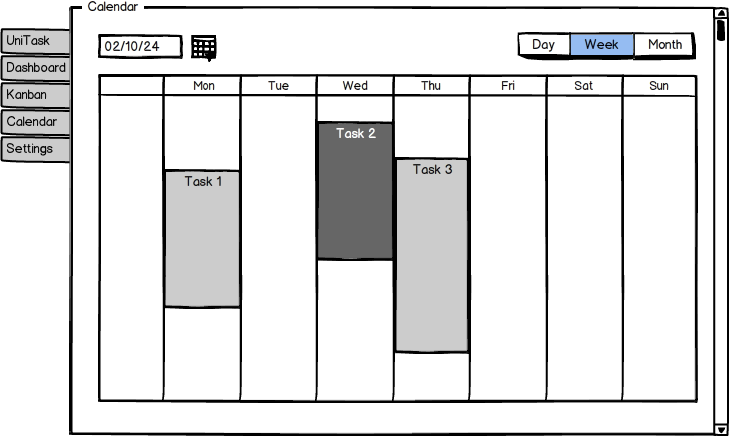
\includegraphics[width=0.65\textwidth]{mockups/Calendar}
%            \caption{\centering Mockup Calendar σελίδας}
%            \label{fig:unitaskMockupCalendar}
%        \end{figure}
%
%        \begin{figure}[p!] \noindent \centering
%            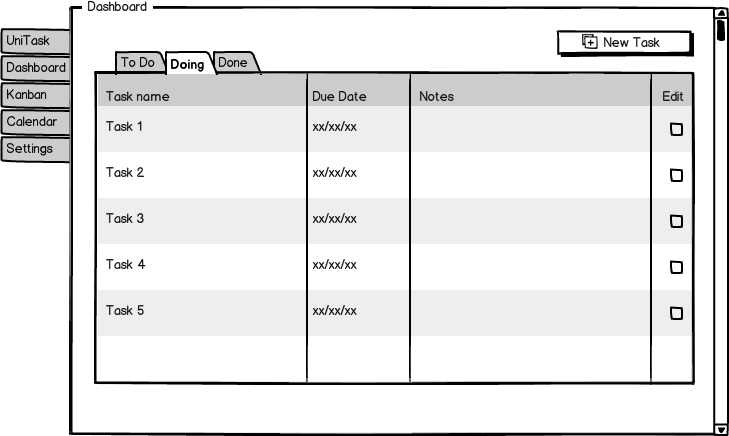
\includegraphics[width=0.65\textwidth]{mockups/Dashboard}
%            \caption{\centering Mockup Dashboard σελίδας}
%            \label{fig:unitaskMockupDashboard}
%        \end{figure}
%
%        \begin{figure}[p!] \noindent \centering
%            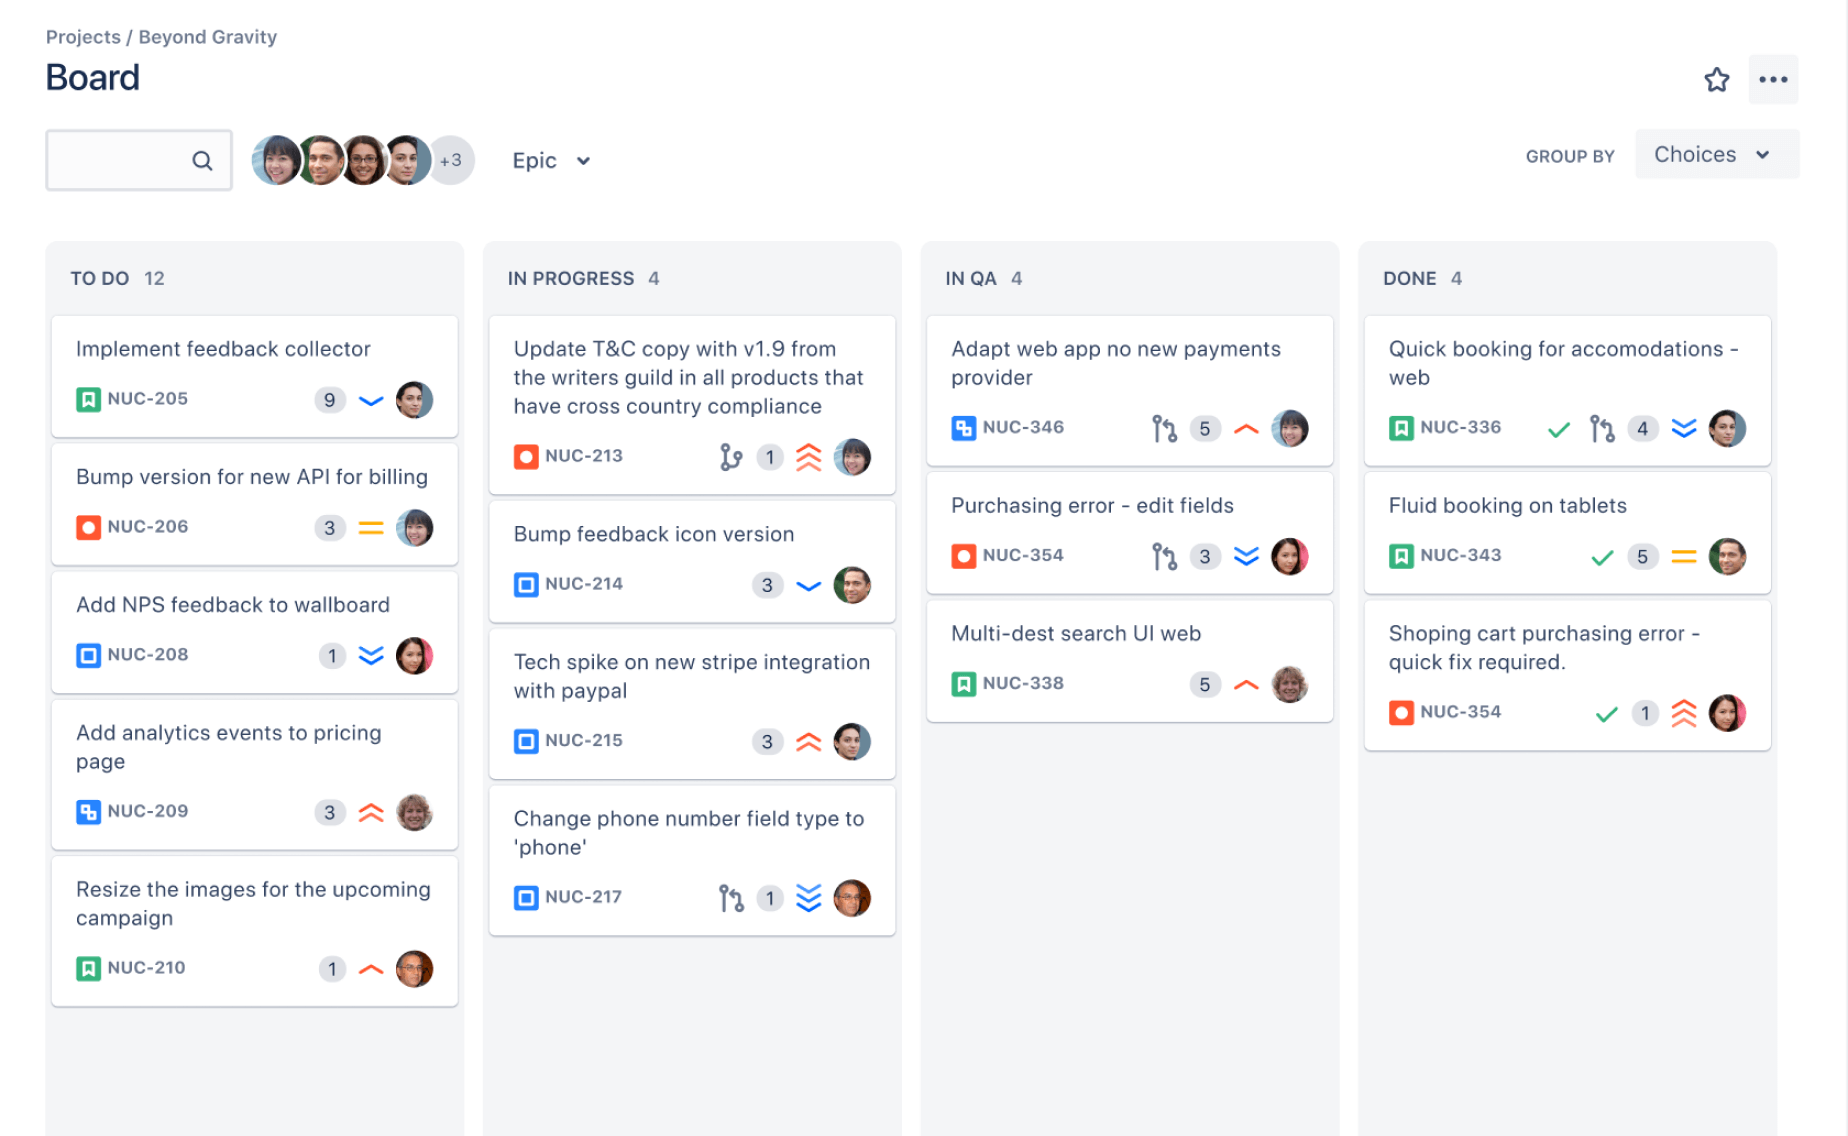
\includegraphics[width=0.65\textwidth]{mockups/Kanban}
%            \caption{\centering Mockup Kanban σελίδας}
%            \label{fig:unitaskMockupKanban}
%        \end{figure}
%
%    \pagebreak
%
%    \section{Η εφαρμογή}
%        Κατά την εκτέλεση της εφαρμογής, είτε τοπικά είτε μέσω της απομακρυσμένης πρόσβασης στο cloud, στη διεύθυνση \texttt{https://unitask-sandbox.mxapps.io/}, εμφανίζεται αρχικά η \textbf{σελίδα σύνδεσης}, όπως φαίνεται στο σχήμα \ref{fig:unitask_Login}. Στη συγκεκριμένη σελίδα, οι χρήστες καλούνται να εισάγουν τα στοιχεία σύνδεσής τους για να αποκτήσουν πρόσβαση στις λειτουργίες της εφαρμογής.
%
%        Ανάλογα με τα στοιχεία σύνδεσης που παρέχονται, το σύστημα διακρίνει δύο επίπεδα πρόσβασης: δικαιώματα διαχειριστή (Administrator) και δικαιώματα χρήστη (User), όπου εκπροσωπούν τους φοιτητές. Οι χρήστες με δικαιώματα Administrator έχουν πρόσβαση σε επιπλέον προηγμένες λειτουργίες διαχείρισης όπως η διαχείριση των χρηστών.
%
%       \begin{figure}[h!] \noindent \centering
%            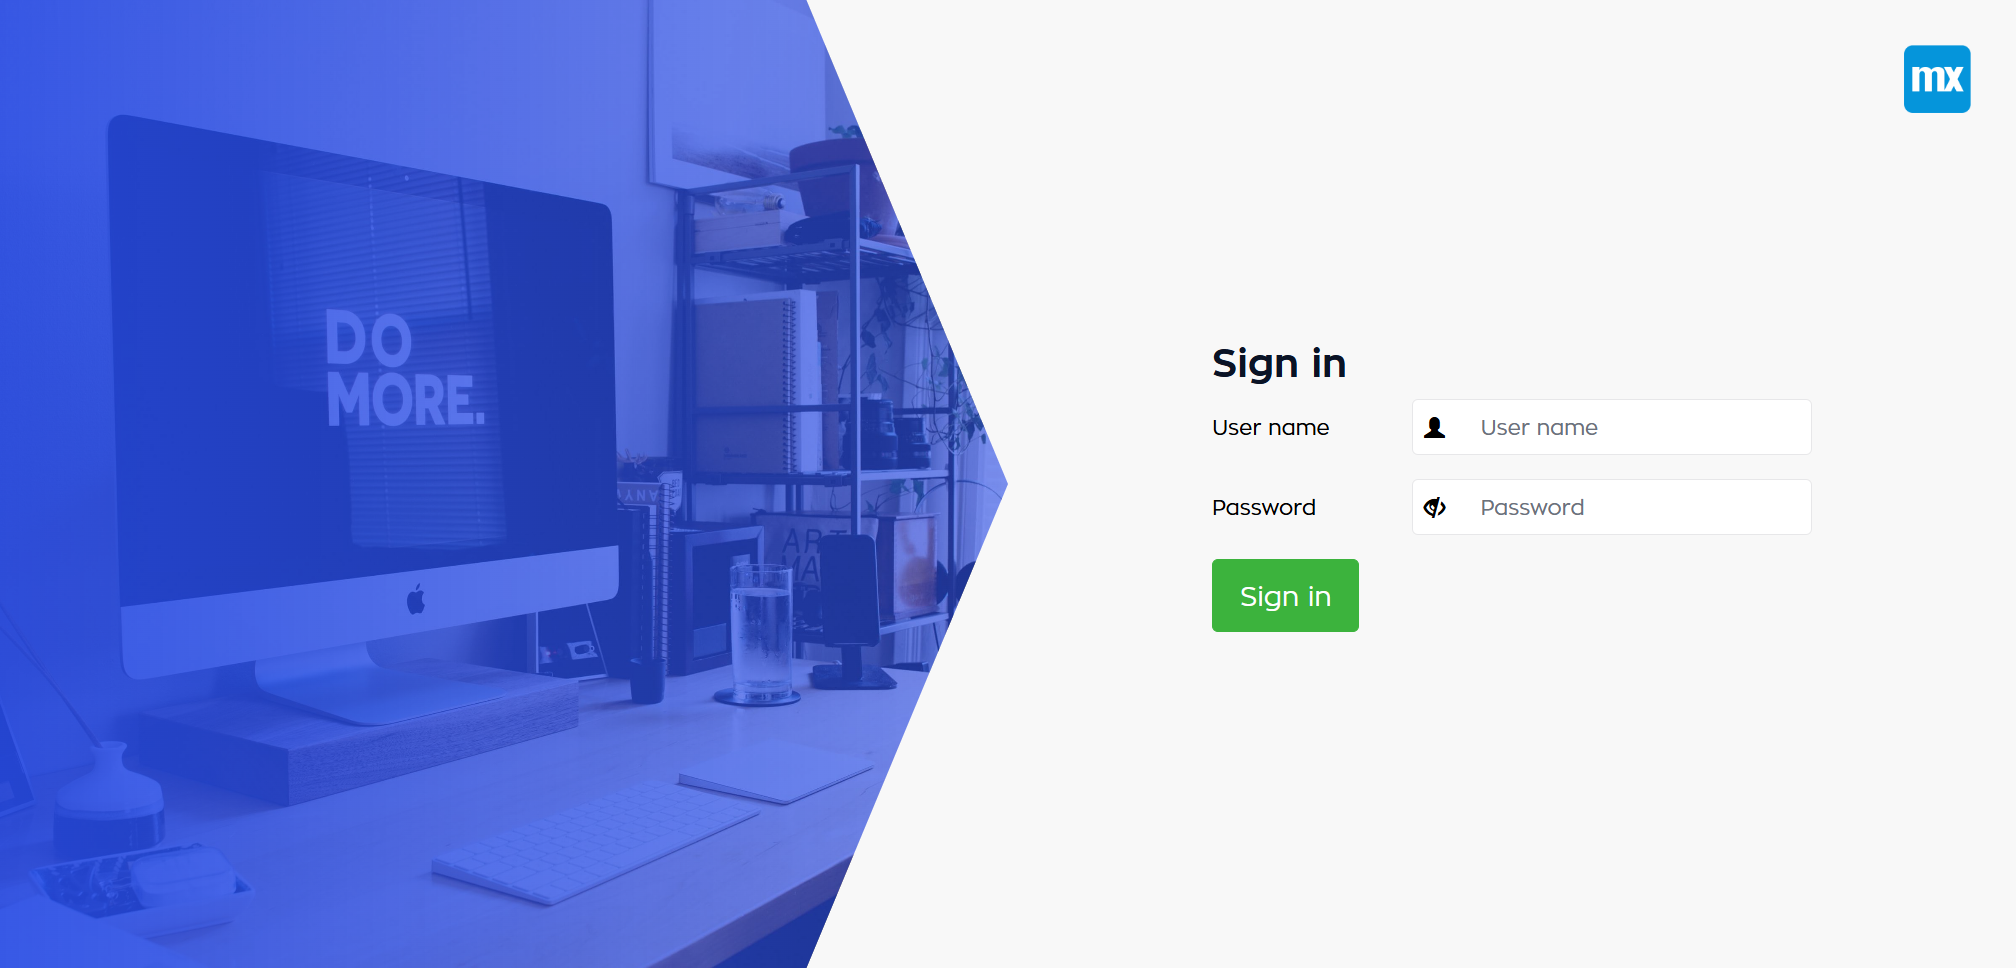
\includegraphics[width=\textwidth]{UniTask/Login}
%            \caption{\centering Σελίδα σύνδεσης}
%            \label{fig:unitask_Login}
%        \end{figure}
%
%        Αρχικά, πραγματοποιείται σύνδεση με τον λογαριασμό διαχειριστή (Administrator) προκειμένου να παρουσιαστούν οι λειτουργίες διαχείρισης χρηστών, συμπεριλαμβανομένης της δυνατότητας προσθήκης νέου χρήστη. Μετά την επιτυχή εισαγωγή των διαπιστευτηρίων του διαχειριστή, τα οποία έχουν οριστεί προκαταβολικά κατά την ανάπτυξη της εφαρμογής (βλ. ενότητα \ref{sec:unitask_mendix}), εμφανίζεται η \textbf{σελίδα διαχείρισης χρηστών}, όπως απεικονίζεται στο σχήμα \ref{fig:unitask_AccountOverview}. Η σελίδα αυτή παρέχει στους διαχειριστές μια ολοκληρωμένη επισκόπηση της λίστας χρηστών της εφαρμογής, καθώς και εργαλεία για τη διαχείρισή τους. Το layout της σελίδας αποτελείται από μια κάθετη μπάρα μενού η οποία περιλαμβάνει τις ίδιες δυνατότητες με τους απλούς χρήστες η οποίες θα αναλυθούν στη συνέχεια.
%
%       \begin{figure}[h!] \noindent \centering
%            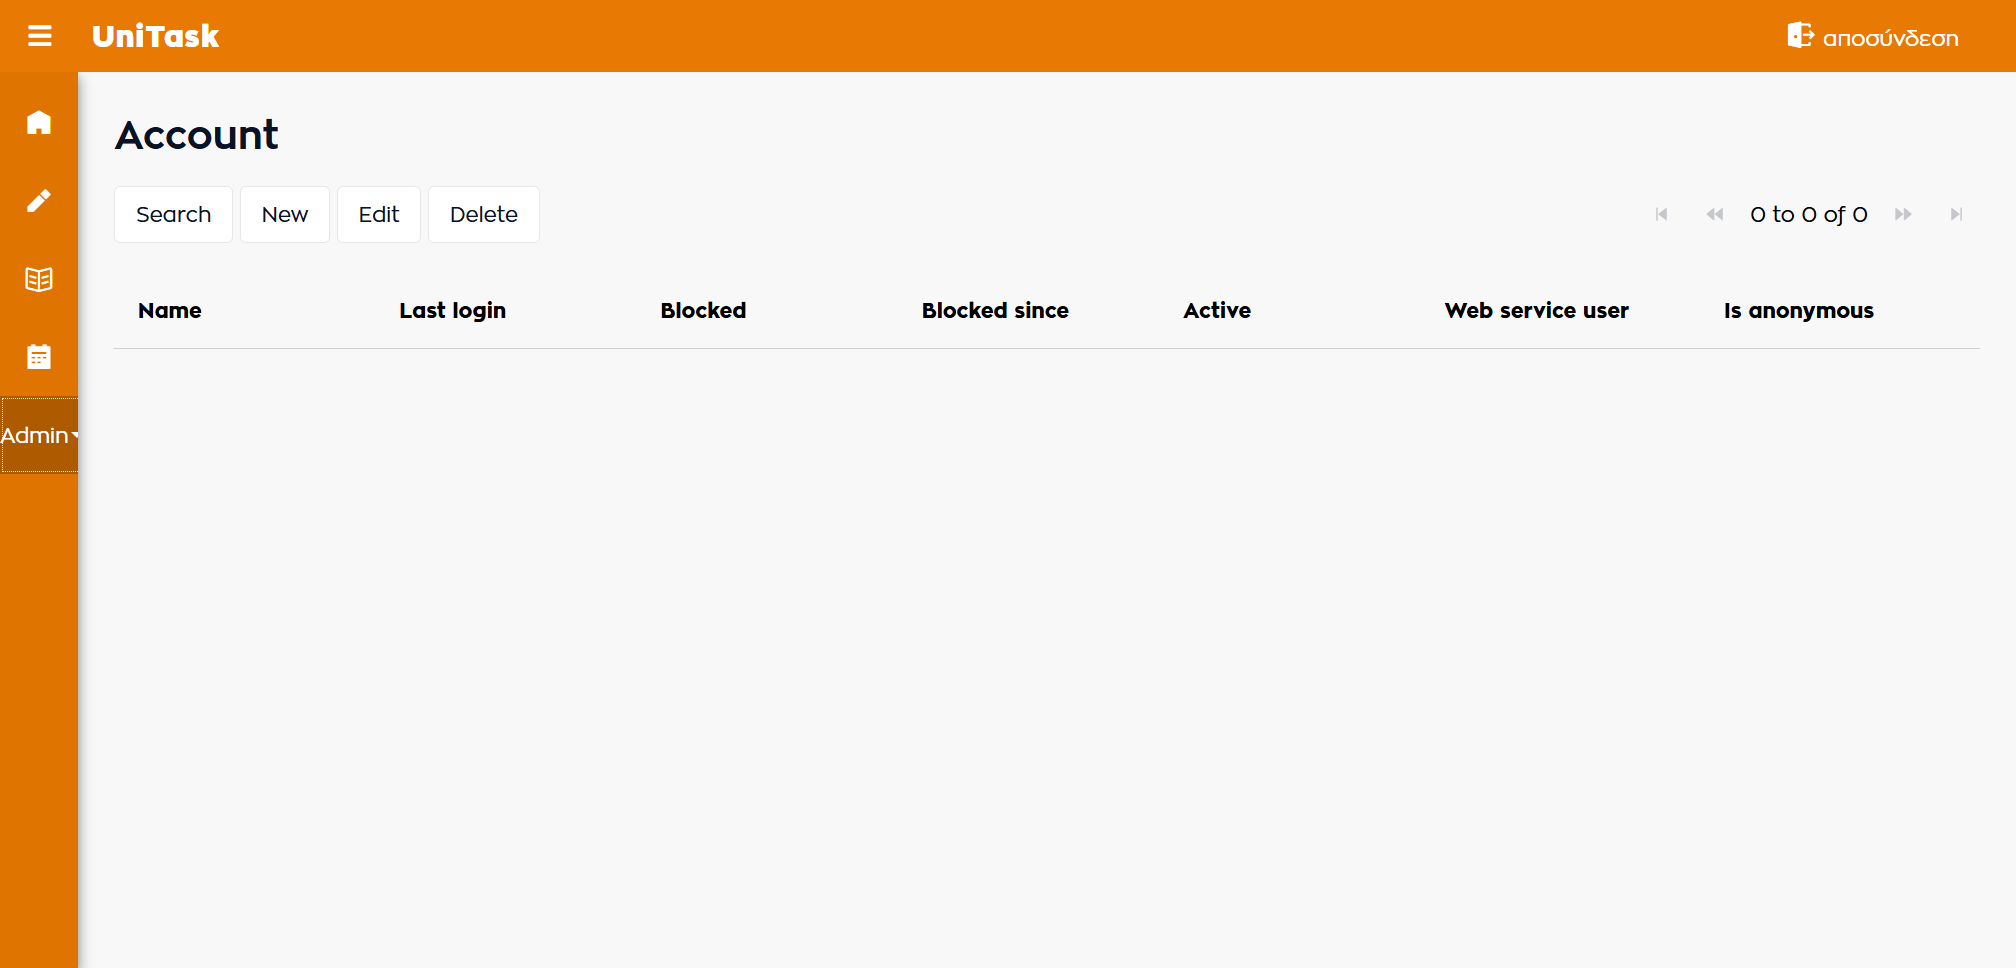
\includegraphics[trim={0 12cm 0 0}, clip, width=\textwidth]{UniTask/AccountOverview}
%            \caption{\centering Σελίδα διαχείρισης χρηστών}
%            \label{fig:unitask_AccountOverview}
%        \end{figure}
%
%        Πατώντας στο κουμπί {\Zona New}, εμφανίζεται η popout σελίδα του σχήματος \ref{fig:unitask_NewAccount} με μια \textbf{φόρμα για την προσθήκη νέου χρήστη}. Η φόρμα περιλαμβάνει πεδία για την εισαγωγή του ονόματος χρήστη ({\Zona Username}), του ρόλου του χρήστη ({\Zona User role}) όπου επιλέγεται αν πρόκειται για προσθήκη διαχειριστή ή χρήστη, του κωδικού πρόσβασης ({\Zona New password} και {\Zona Confirm password}). Λόγω του ότι ο χρήστης User έχει κληρονομήσει γνωρίσματα από την κλάση \texttt{System.User} του Mendix, έχουν προστεθεί πεδία όπως το {\Zona Blocked}, η οποία γίνεται αληθής μετά από κάποιες αποτυχημένες προσπάθειες σύνδεσης, το {\Zona Active} που γίνεται αληθές όταν ο χρήστης συνδεθεί, το {\Zona Time zone} όπου ορίζεται η ζώνη ώρας του χρήστη και το {\Zona Language} όπου ορίζεται η γλώσσα του χρήστη.
%
%        \begin{figure}[h!] \noindent \centering
%            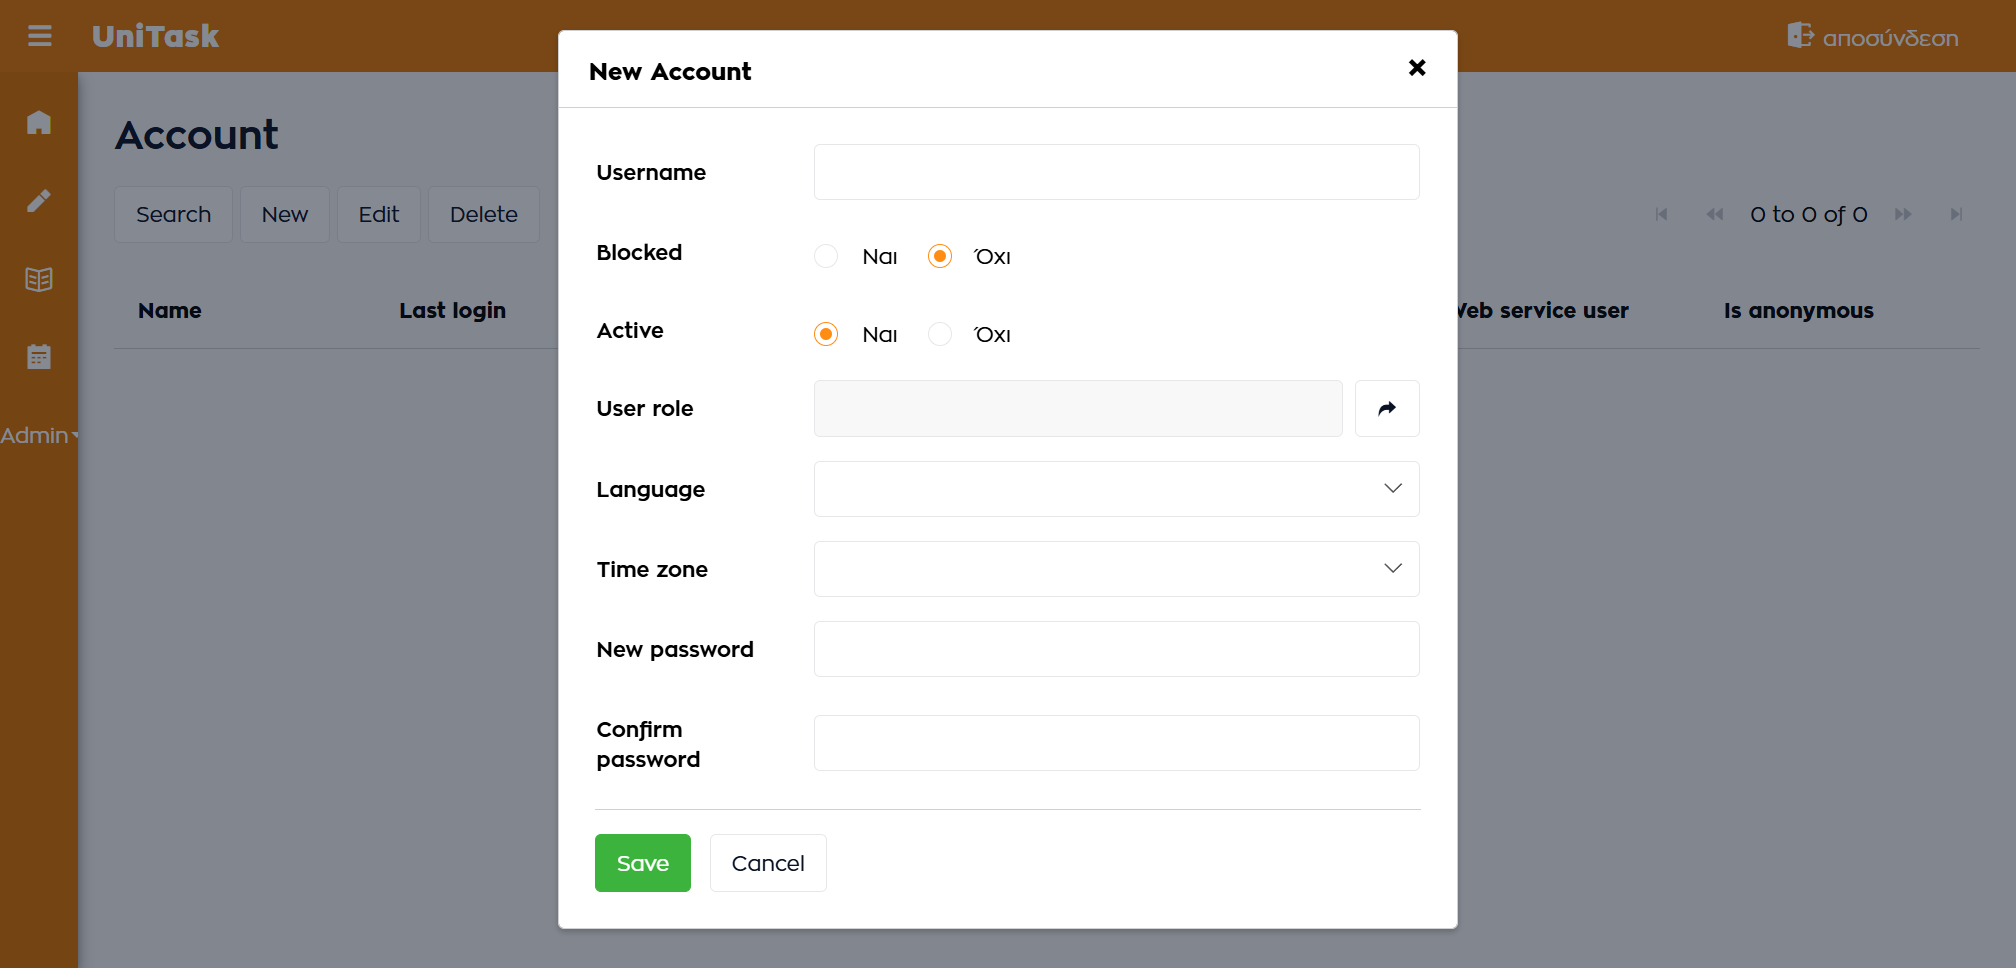
\includegraphics[width=\textwidth]{UniTask/NewAccount}
%            \caption{\centering Φόρμα προσθήκης νέου χρήστη}
%            \label{fig:unitask_NewAccount}
%        \end{figure}
%
%        Δημιουργούμε έναν χρήστη με όνομα \texttt{Foithths}, ο οποίος εμφανίζεται στη λίστα των χρηστών (σχήμα \ref{fig:unitask_AccountOverview_WithStudent}. Πατώντας στο όνομά του, εμφανίζεται η σελίδα επεξεργασίας του χρήστη, όπως φαίνεται στο σχήμα \ref{fig:unitask_EditAccount}. Στη λίστα των χρηστών υπάρχει η δυνατότητα αναζήτησης χρηστών βάσει όλων των στοιχείων τους (σχήμα \ref{fig:unitask_SearchAccounts}), όπως επίσης και η δυνατότητα διαγραφής τους.
%
%        \begin{figure}[h!] \noindent \centering
%            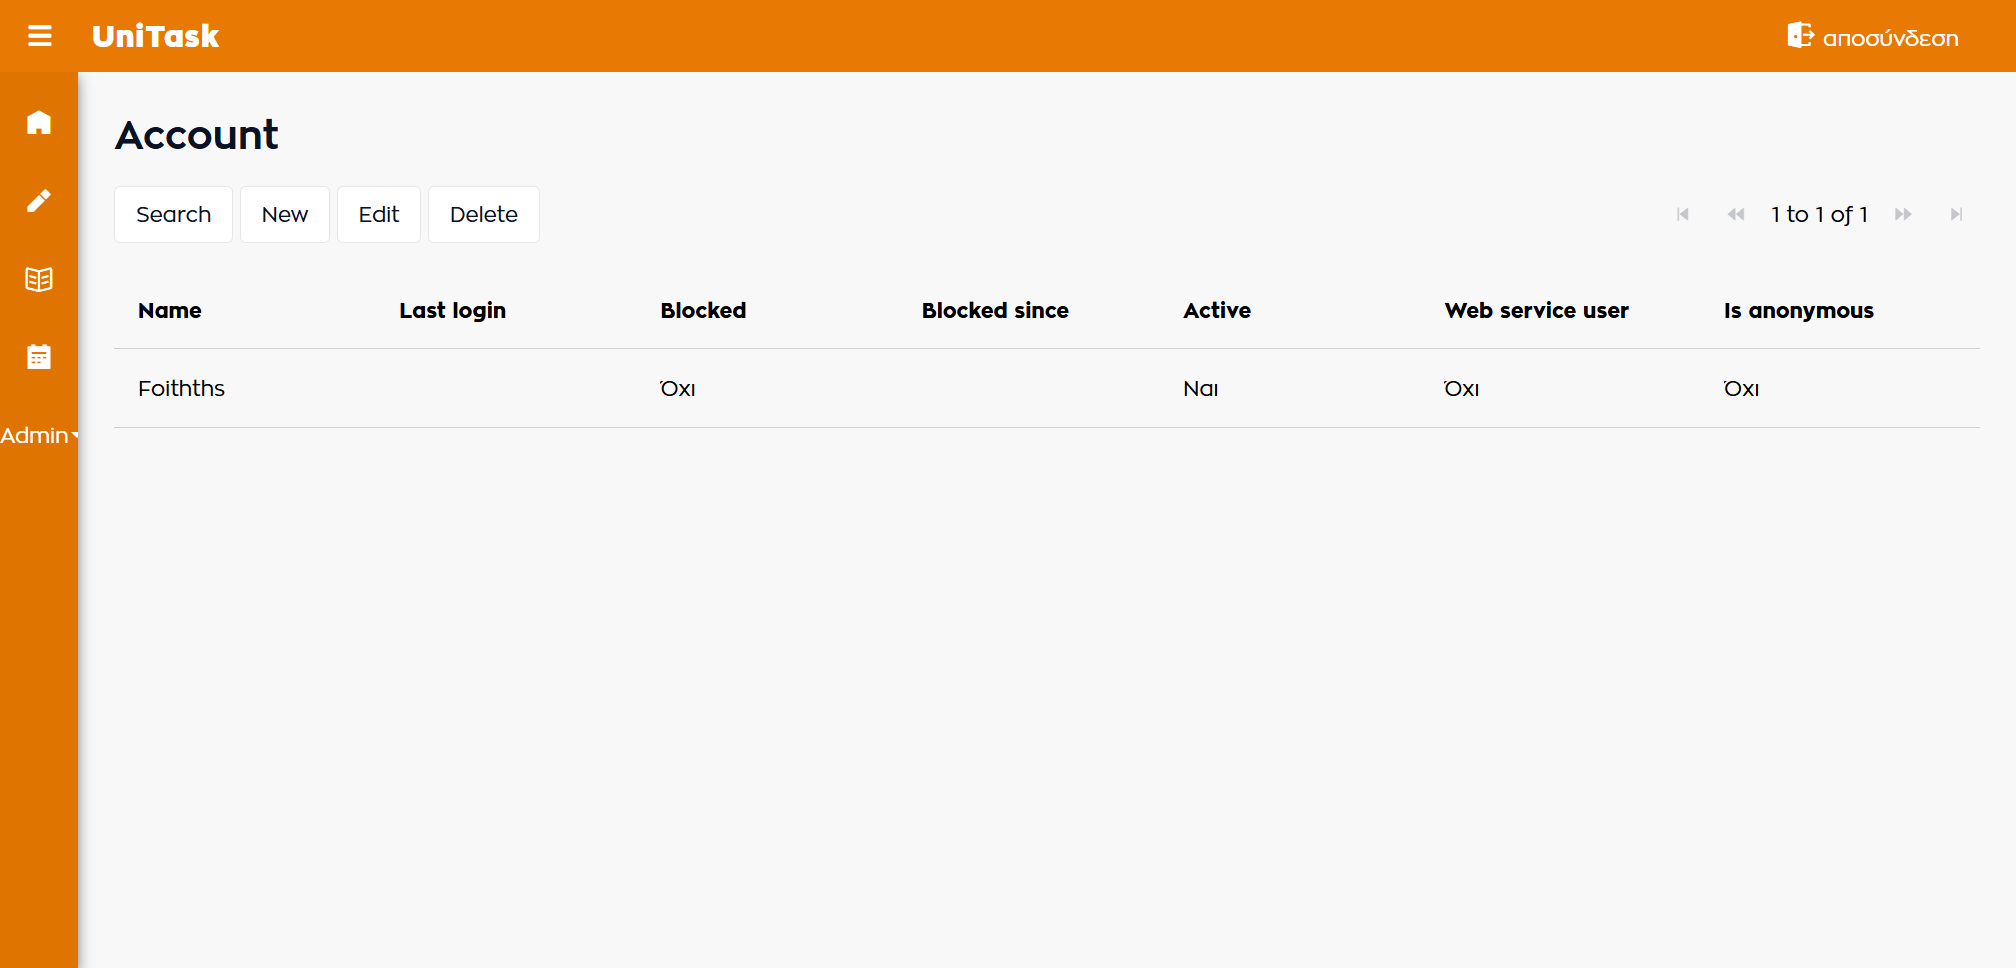
\includegraphics[trim={0 17cm 0 0}, clip, width=\textwidth]{UniTask/AccountOverview_WithStudent}
%            \caption{\centering Λίστα χρηστών με τον χρήστη \texttt{Foithths}}
%            \label{fig:unitask_AccountOverview_WithStudent}
%        \end{figure}
%
%        \begin{figure}[h!] \noindent \centering
%            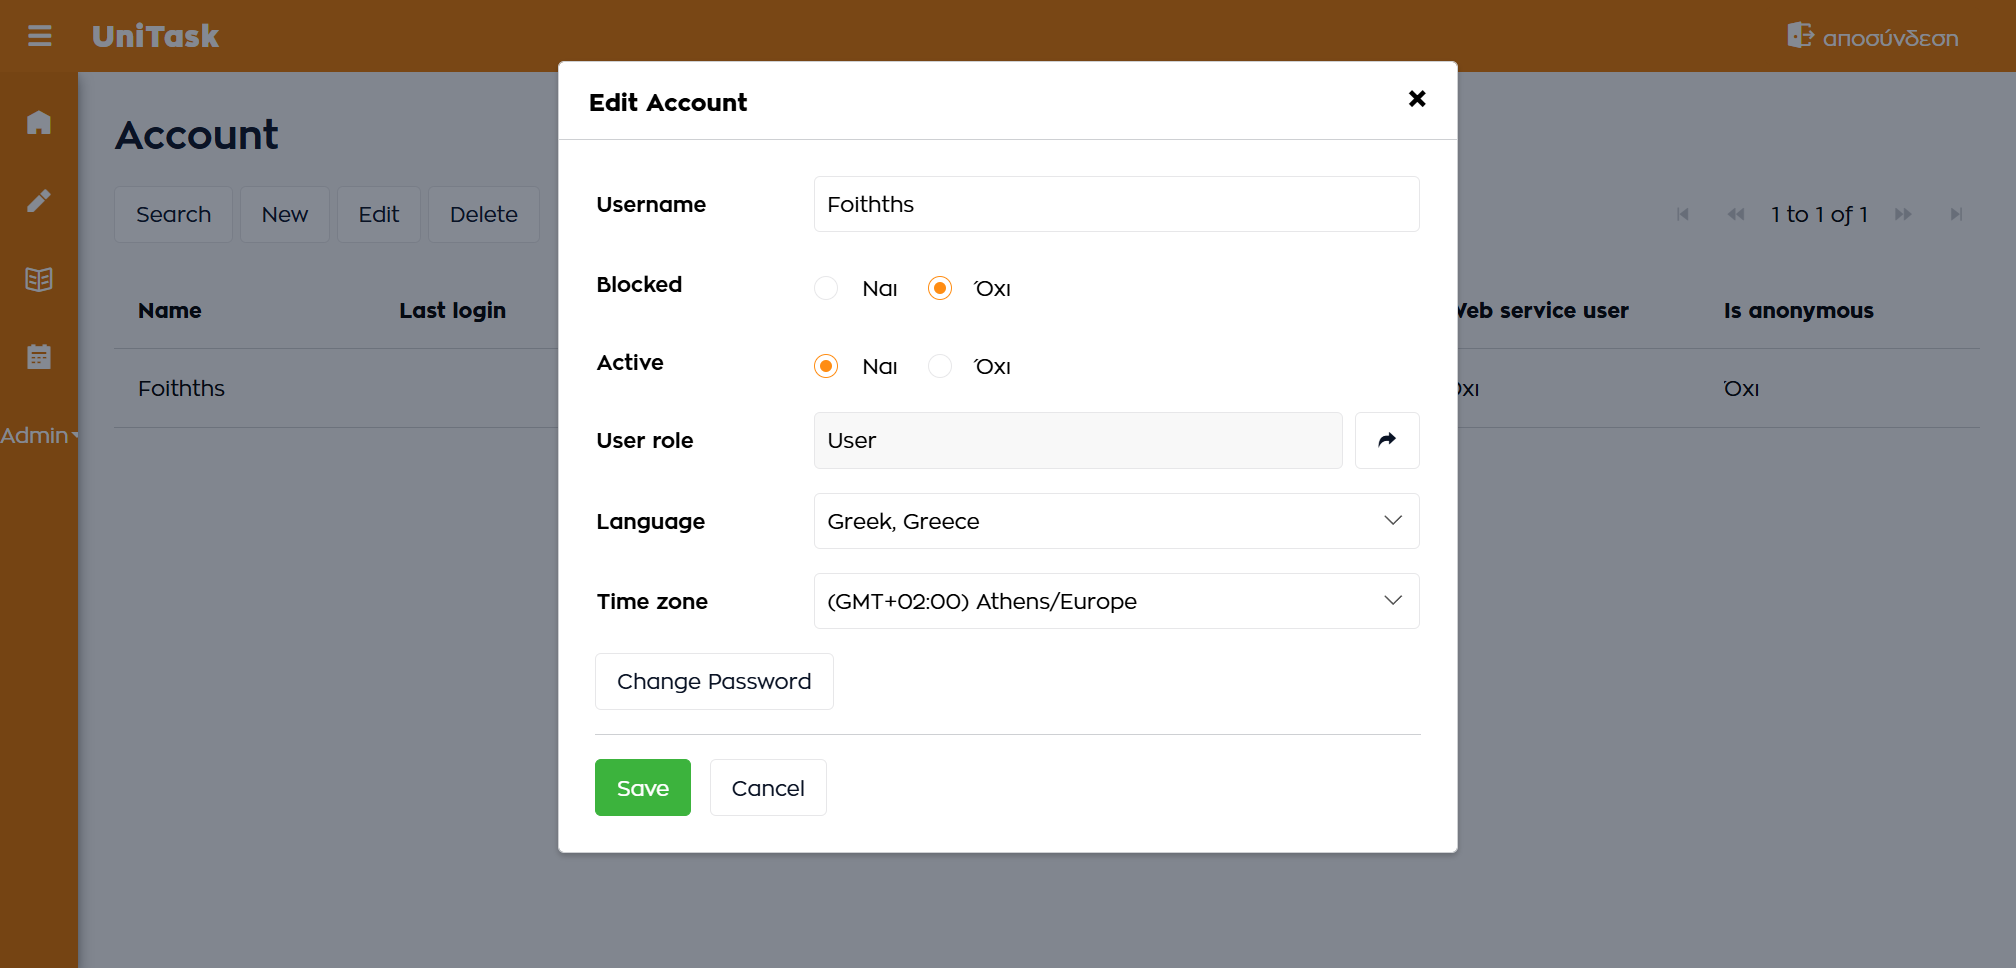
\includegraphics[trim={0 3cm 0 0}, clip, width=\textwidth]{UniTask/EditAccount}
%            \caption{\centering Επεξεργασία στοιχείων χρήστη}
%            \label{fig:unitask_EditAccount}
%        \end{figure}
%
%        \begin{figure}[h!] \noindent \centering
%            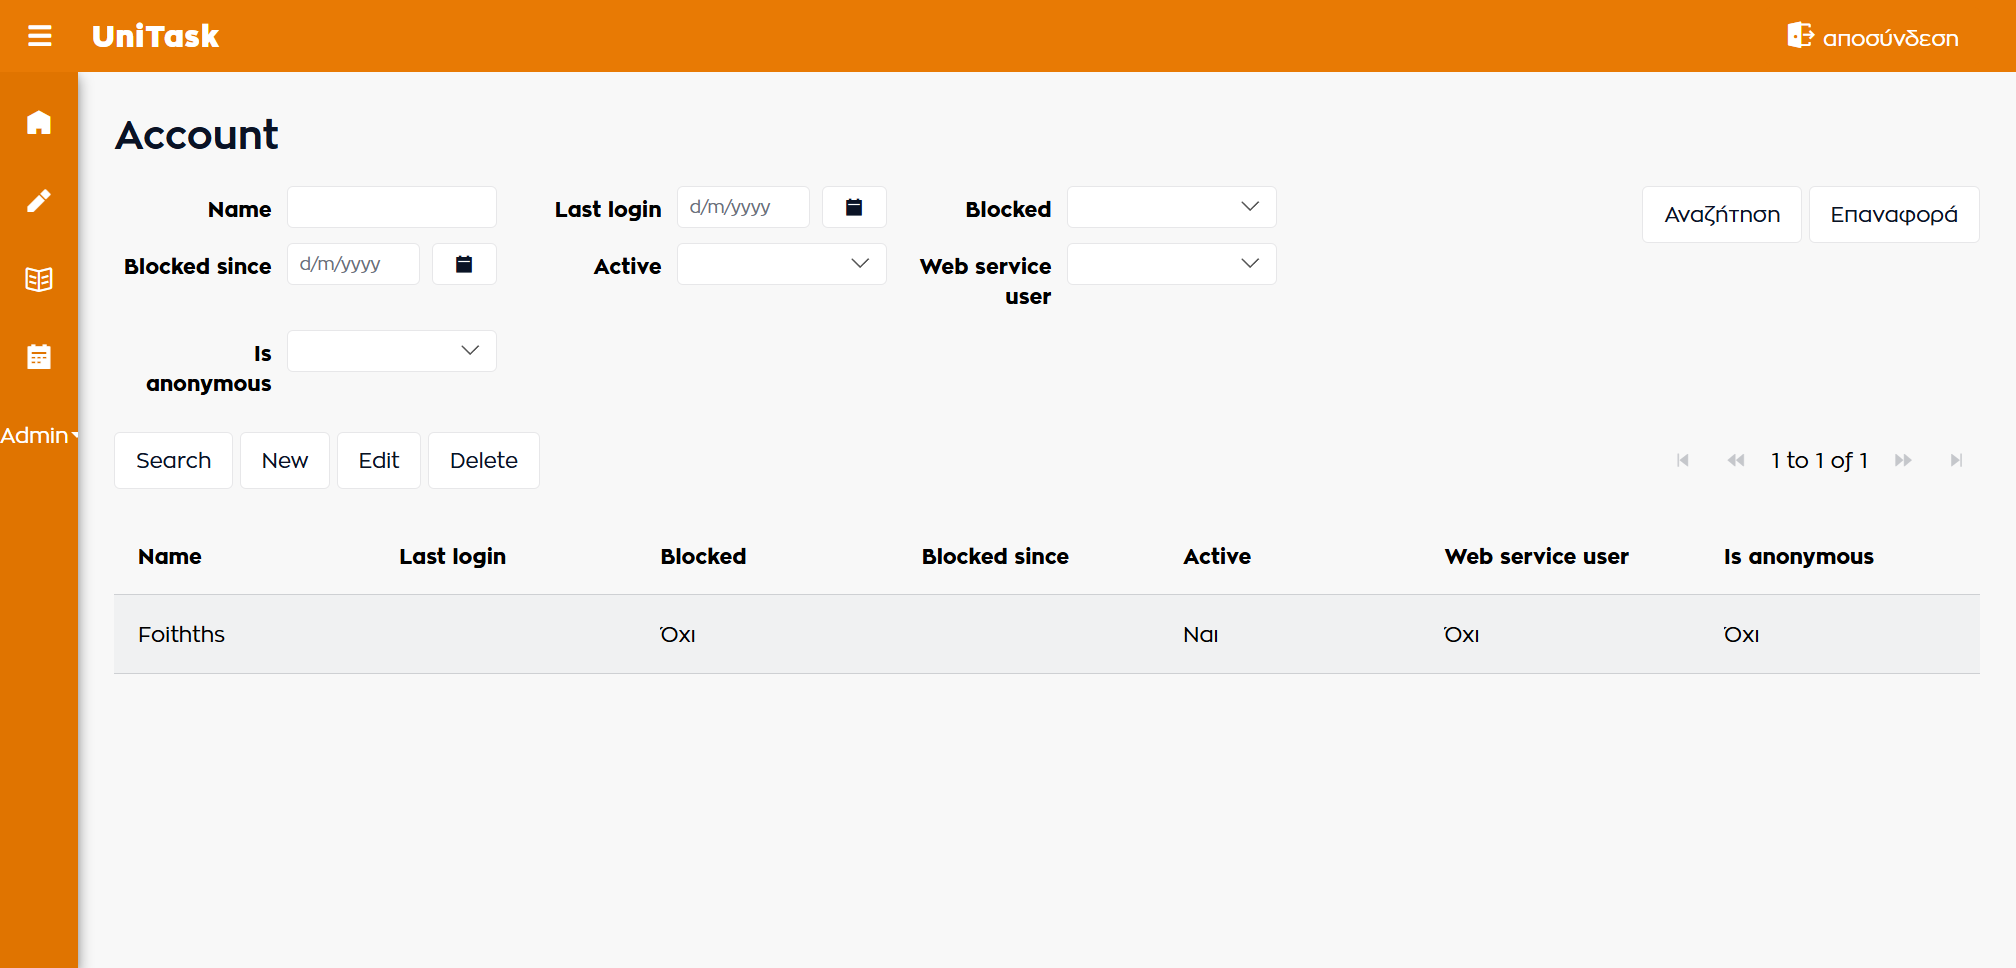
\includegraphics[trim={0 7cm 0 0}, clip, width=\textwidth]{UniTask/SearchAccounts}
%            \caption{\centering Αναζήτηση χρήστη}
%            \label{fig:unitask_SearchAccounts}
%        \end{figure}
%
%        Αφού αποσυνδεθούμε και συνδεθούμε ως \texttt{Foithths}, μας υποδέχεται η \textbf{αρχική σελίδα} της εφαρμογής (σχήμα \ref{fig:unitask_Home}). Η σελίδα περιλαμβάνει ένα κεντρικό call to action κουμπί ({\Zona όλες οι εργασίες}) το οποίο οδηγεί στο {\Zona dashboard}.
%
%        \begin{figure}[h!] \noindent \centering
%            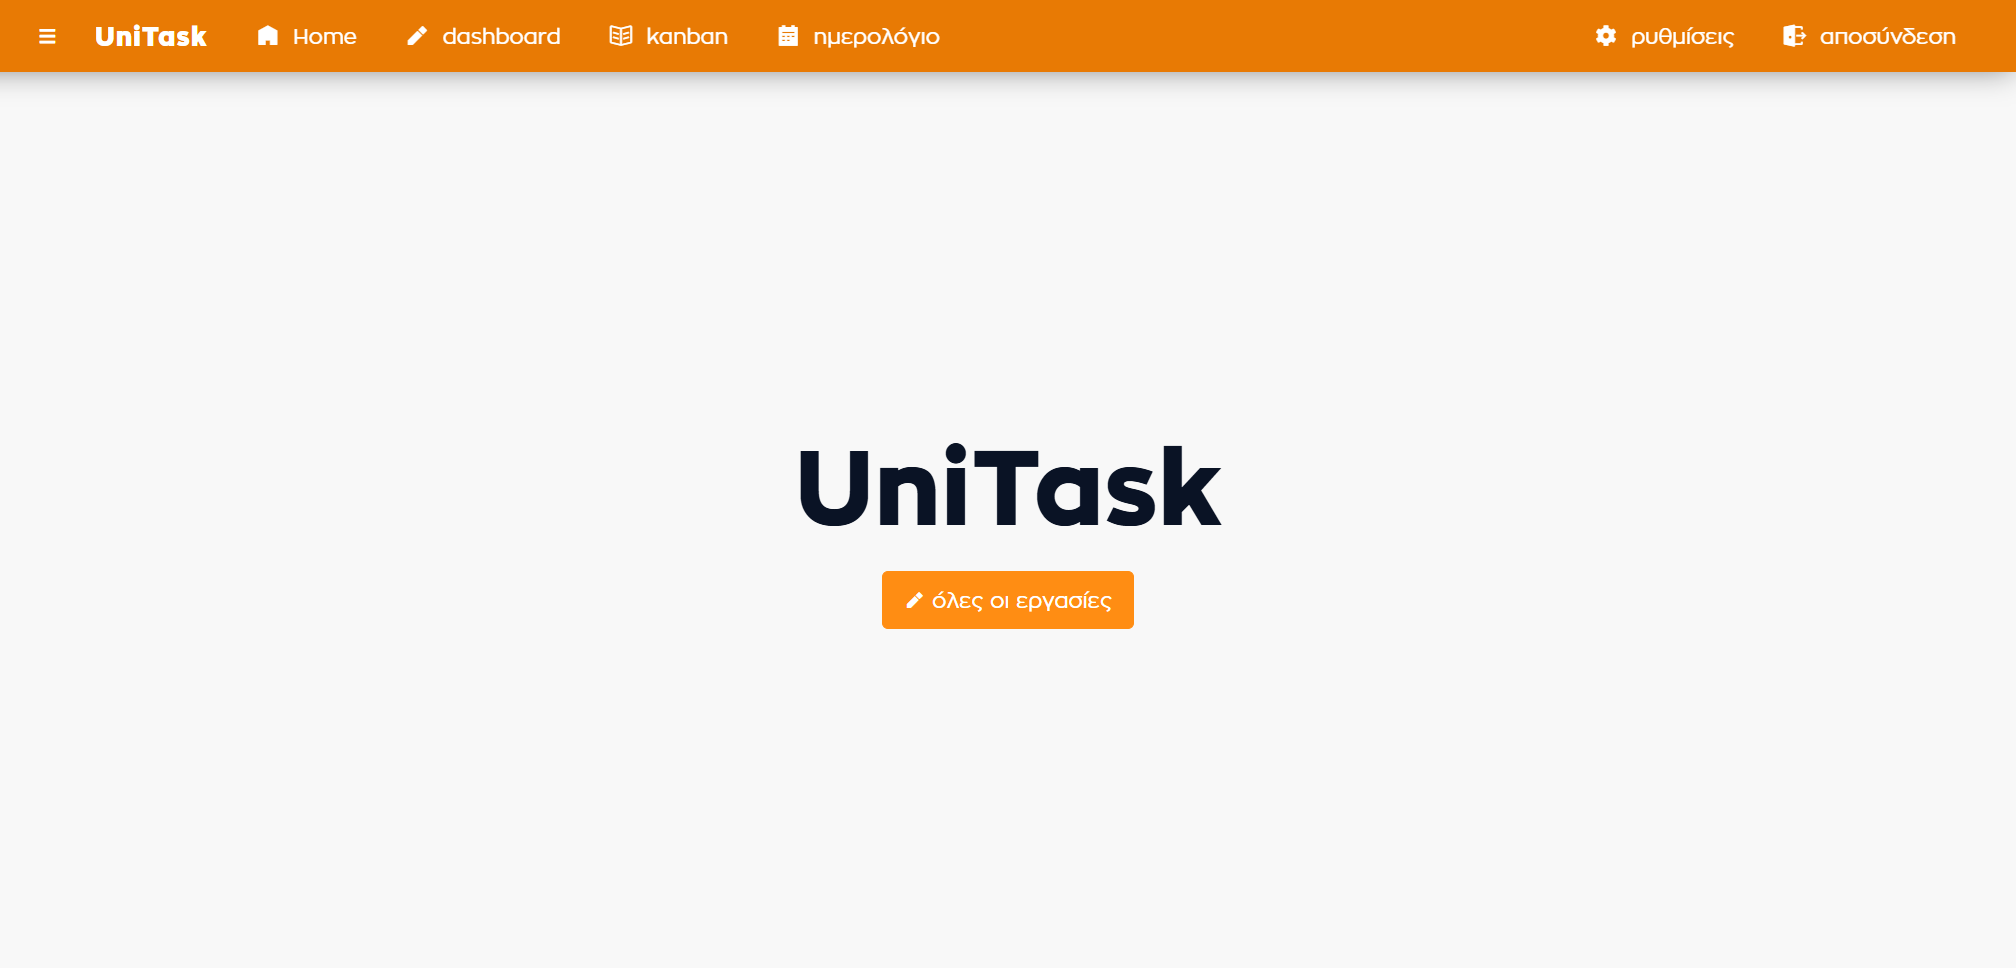
\includegraphics[width=\textwidth]{UniTask/Home}
%            \caption{\centering Αρχική σελίδα εφαρμογής}
%            \label{fig:unitask_Home}
%        \end{figure}
%
%        \begin{figure}[h!] \noindent \centering
%            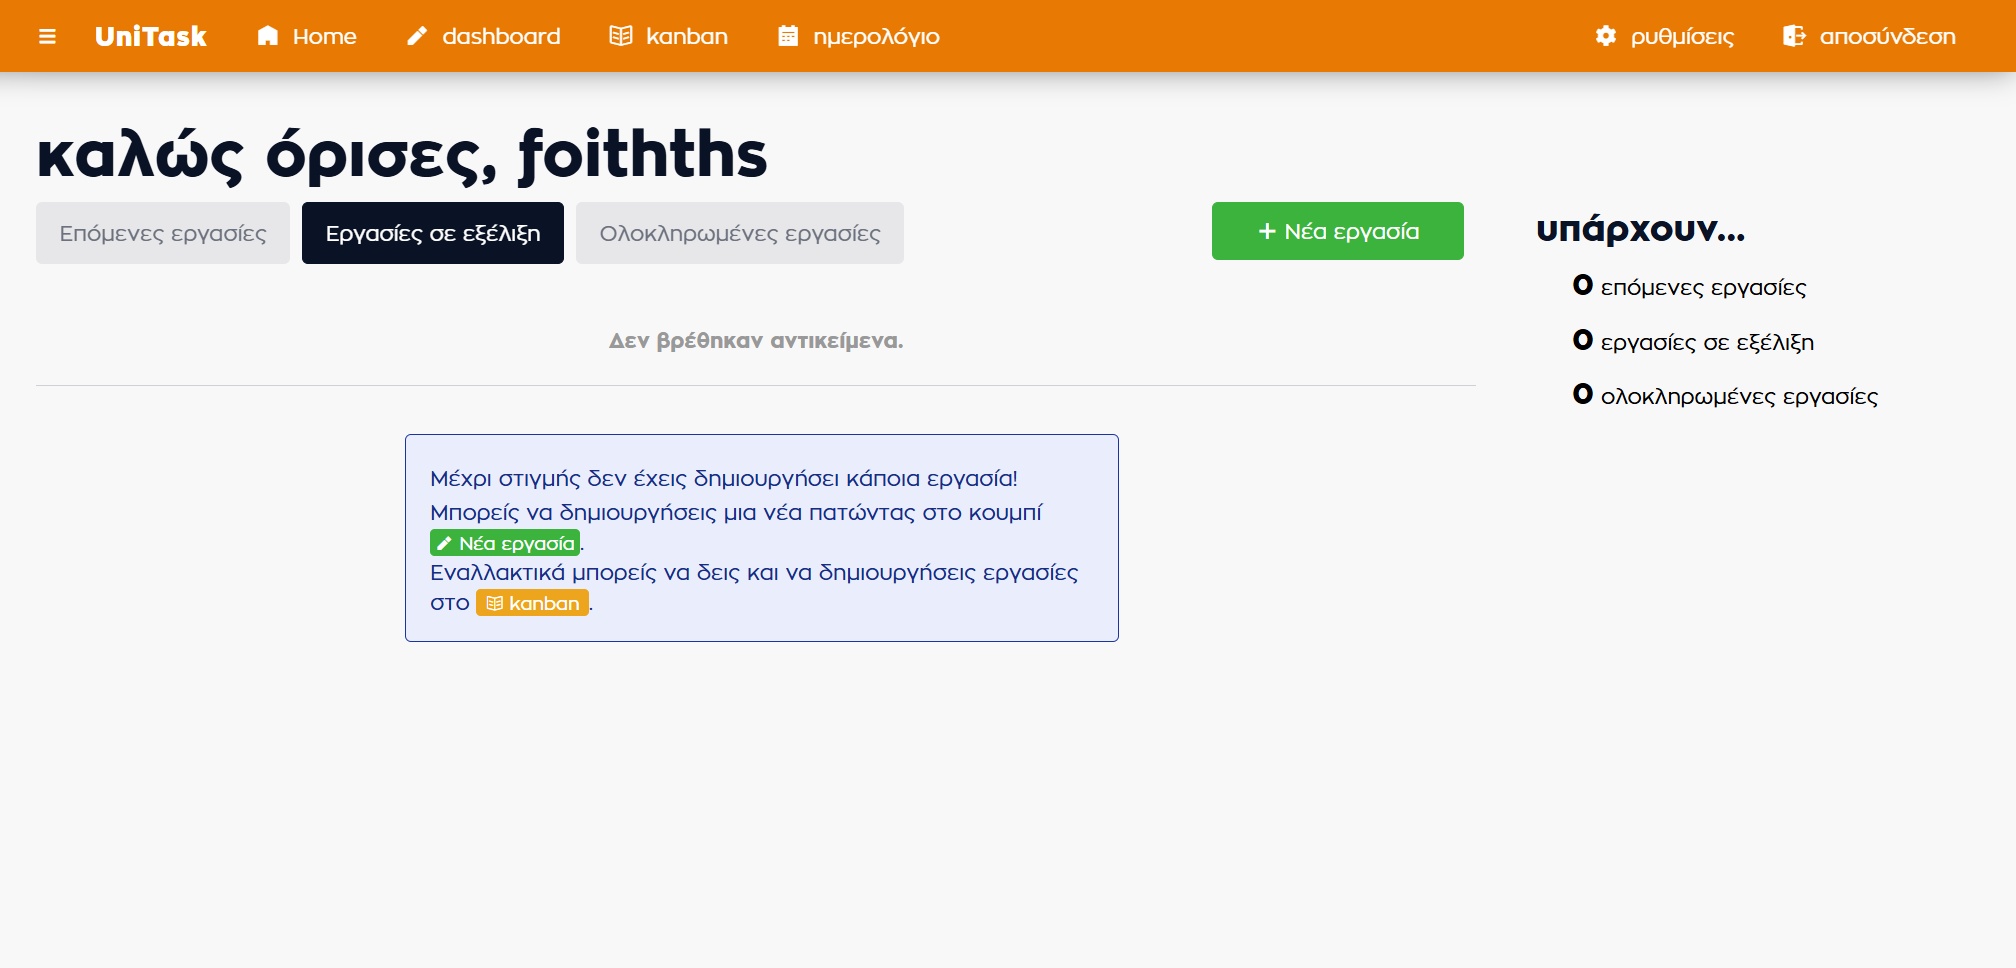
\includegraphics[width=\textwidth]{UniTask/TaskDashboard}
%            \caption{\centering Dashboard εργασιών}
%            \label{fig:unitask_TaskDashboard}
%        \end{figure}
%
%        Στο σχήμα \ref{fig:unitask_TaskDashboard} εμφανίζεται η σελίδα {\ZonaSB dashboard}. Πρόκειται για την κεντρική σελίδα προβολής, δημιουργίας και επεξεργασίας των εργασιών του χρήστη. Περιλαμβάνονται τρεις καρτέλες ({\Zona Επόμενες εργασίες}, {\Zona Εργασίες σε εξέλιξη}, {\Zona Ολοκληρωμένες εργασίες}). Οι επόμενες εργασίες αφορούν εργασίες που έχουν σκοπό να πραγματοποιηθούν στο άμεσο μέλλον αλλά όχι τη δεδομένη χρονική στιγμή, οι εργασίες σε εξέλιξη αφορούν εργασίες που βρίσκονται σε εξέλιξη και οι ολοκληρωμένες εργασίες αφορούν εργασίες που έχουν ολοκληρωθεί.
%
%        Στη σελίδα επίσης περιλαμβάνεται ένα επεξηγηματικό παράθυρο που εμφανίζεται μόνο όταν ο χρήστης δεν έχει δημιουργήσει κάποια εργασία και του εξηγεί το τρόπο λειτουργίας της εφαρμογής. Στο {\Zona dashboard} επίσης περιλαμβάνονται μετρητές για το σύνολο των εργασιών που υπάρχουν ανά κατηγορία, όπως επίσης και ένα κεντρικό κουμπί δημιουργίας εργασιών ({\Zona Νέα εργασία}).
%
%        \begin{figure}[h!] \noindent \centering
%            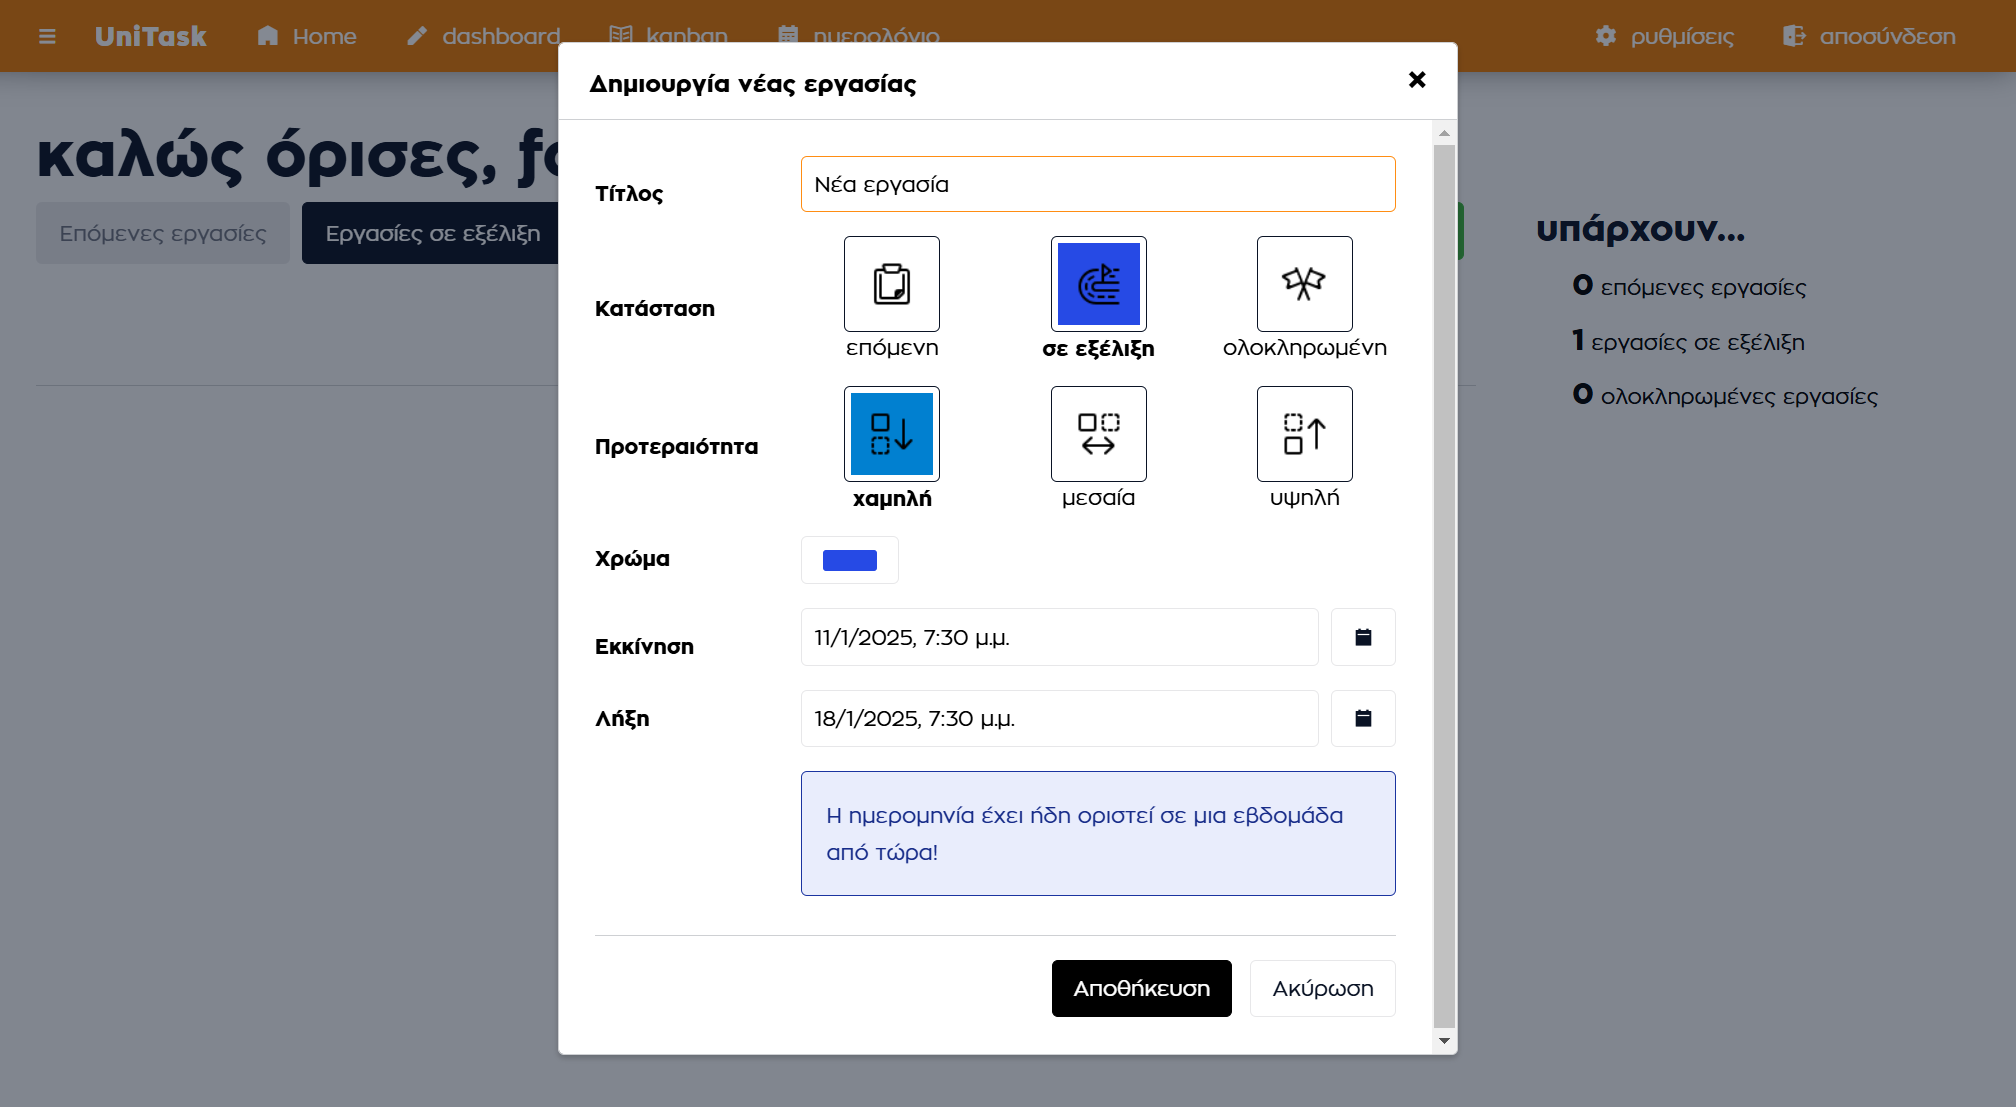
\includegraphics[width=\textwidth]{UniTask/NewTask_Default}
%            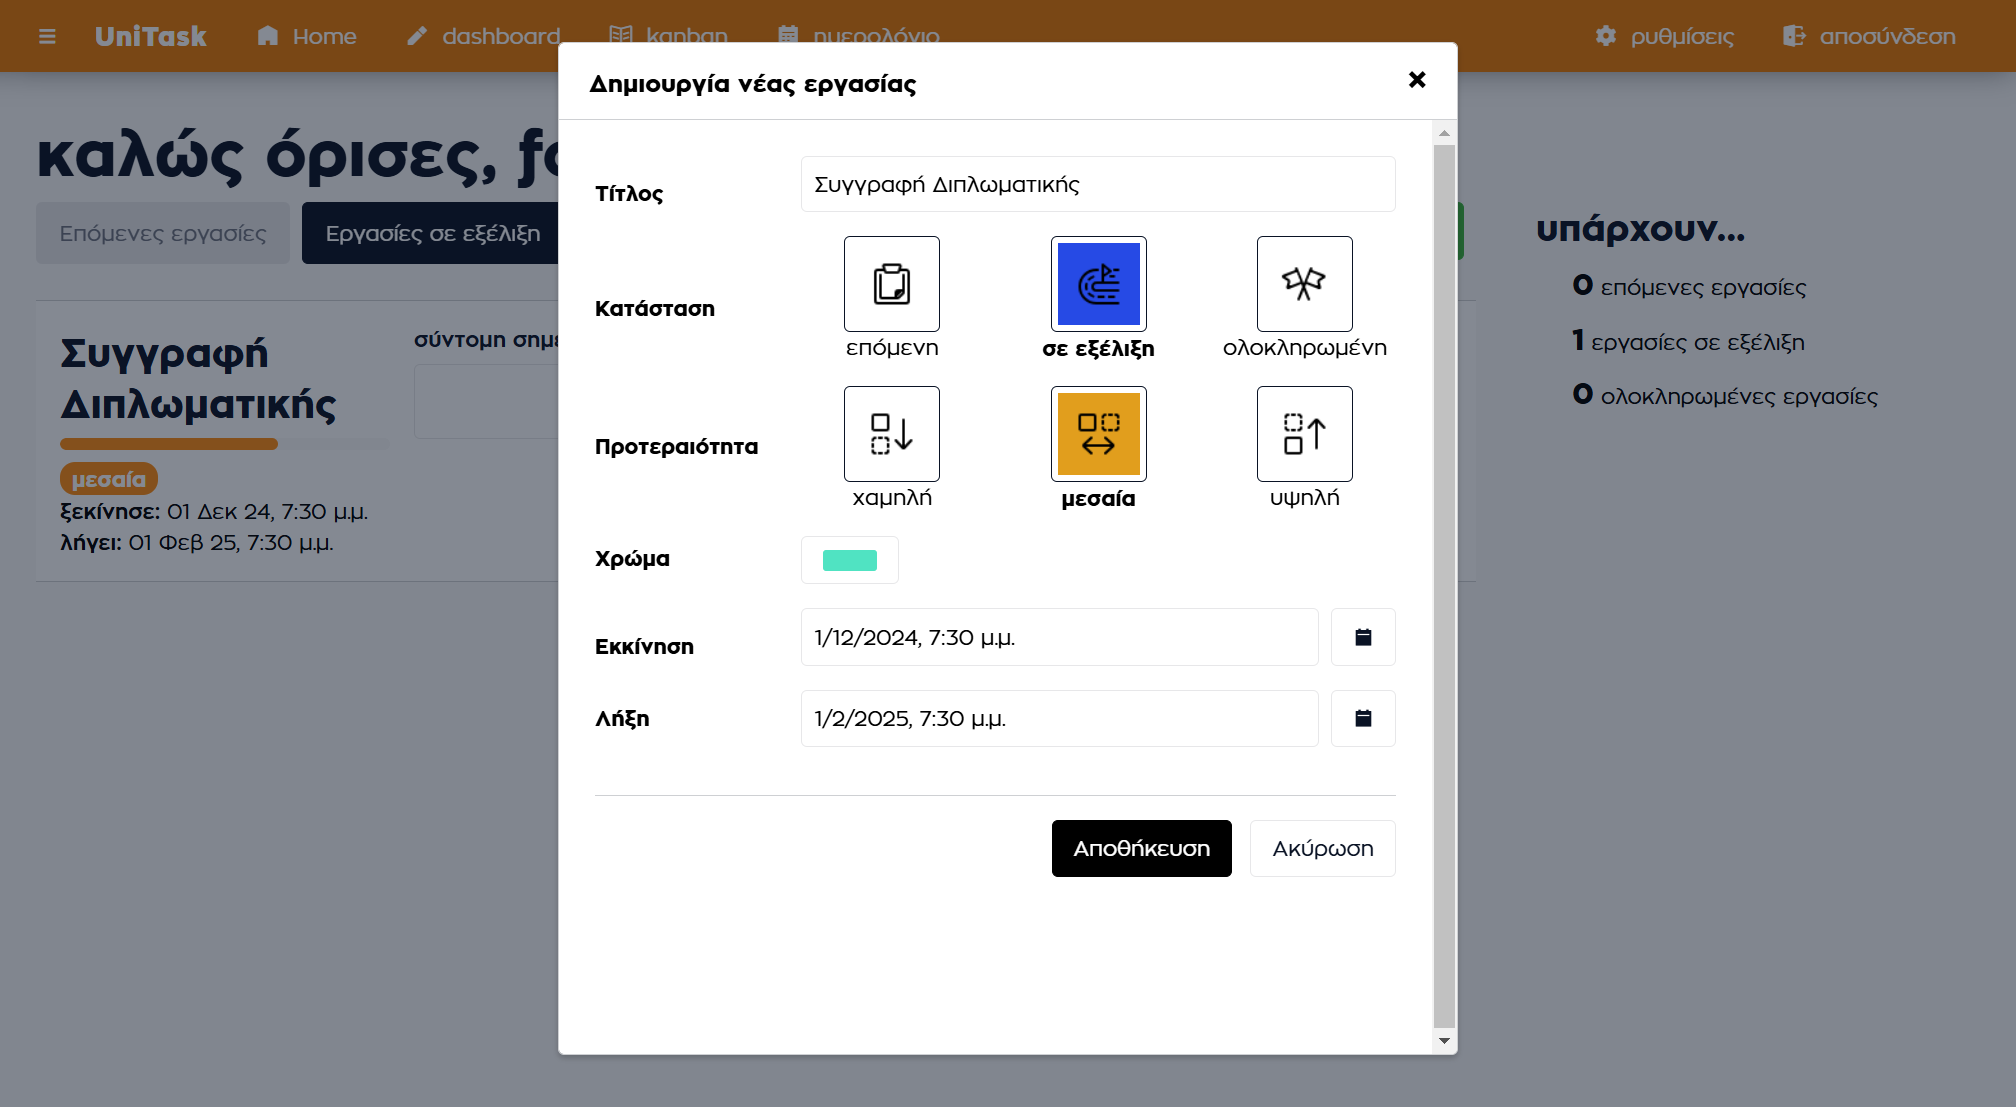
\includegraphics[width=\textwidth]{UniTask/NewTask_Finished}
%            \caption{\centering Δημιουργία νέας εργασίας}
%            \label{fig:unitask_NewTask}
%        \end{figure}
%
%        Πατώντας το, εμφανίζεται ένα popout παράθυρο (σχήμα \ref{fig:unitask_NewTask}.1) με μια φόρμα για τη δημιουργία μιας νέας εργασίας. Η φόρμα αυτή περιλαμβάνει πεδία για την εισαγωγή του τίτλου της εργασίας ({\Zona Τίτλος}), της ημερομηνίας έναρξης ({\Zona Εκκίνηση}) και λήξης ({\Zona Λήξη}), της κατάστασης της εργασίας ({\Zona Κατάσταση}), της προτεραιότητας της εργασίας ({\Zona Προτεραιότητα}) όπως επίσης και του χρώματος της εργασίας ({\Zona Χρώμα}), όπως θα αποτυπωθεί μετέπειτα στο ημερολόγιο. Στο popout παράθυρο ορίζεται προεπιλεγμένα ως ημερομηνία λήξης της εργασίας μια εβδομάδα μετέπειτα από την ημερομηνία δημιουργίας της, ενώ η κατάσταση της εργασίας έχει προκαθοριστεί (γίνεται να τροποποιηθεί φυσικά) ανάλογα με το ποια καρτέλα ήταν ανοιχτή στο dashboard. Αφού επεξεργαστούμε το παράθυρο όπως επιθυμούμε (σχήμα \ref{fig:unitask_NewTask}.2), πατάμε αποθήκευση για την αποθήκευση της εργασίας.
%
%        Να σημειωθεί πως οι επιλογές που αφορούν την κατάσταση και την προτεραιότητα της εργασίας είναι χρωματικά ταξινομημένες (color-coded) με το δικό τους γραφικό σύμβολο, όπως φαίνεται στο σχήμα \ref{fig:unitask_NewTask_AllOptions}, με σκοπό να διευκολύνει τον χρήστη για την άμεση αναγνώριση τους.
%
%        \begin{figure}[h!] \noindent \centering
%            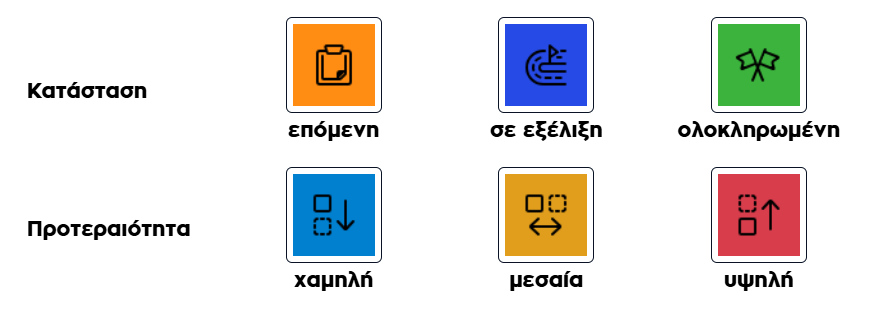
\includegraphics[width=0.7\textwidth]{UniTask/NewTask_AllOptions}
%            \caption{\centering Επιλογές κατάστασης και προτεραιότητας εργασίας}
%            \label{fig:unitask_NewTask_AllOptions}
%        \end{figure}
%
%        \begin{figure}[h!] \noindent \centering
%            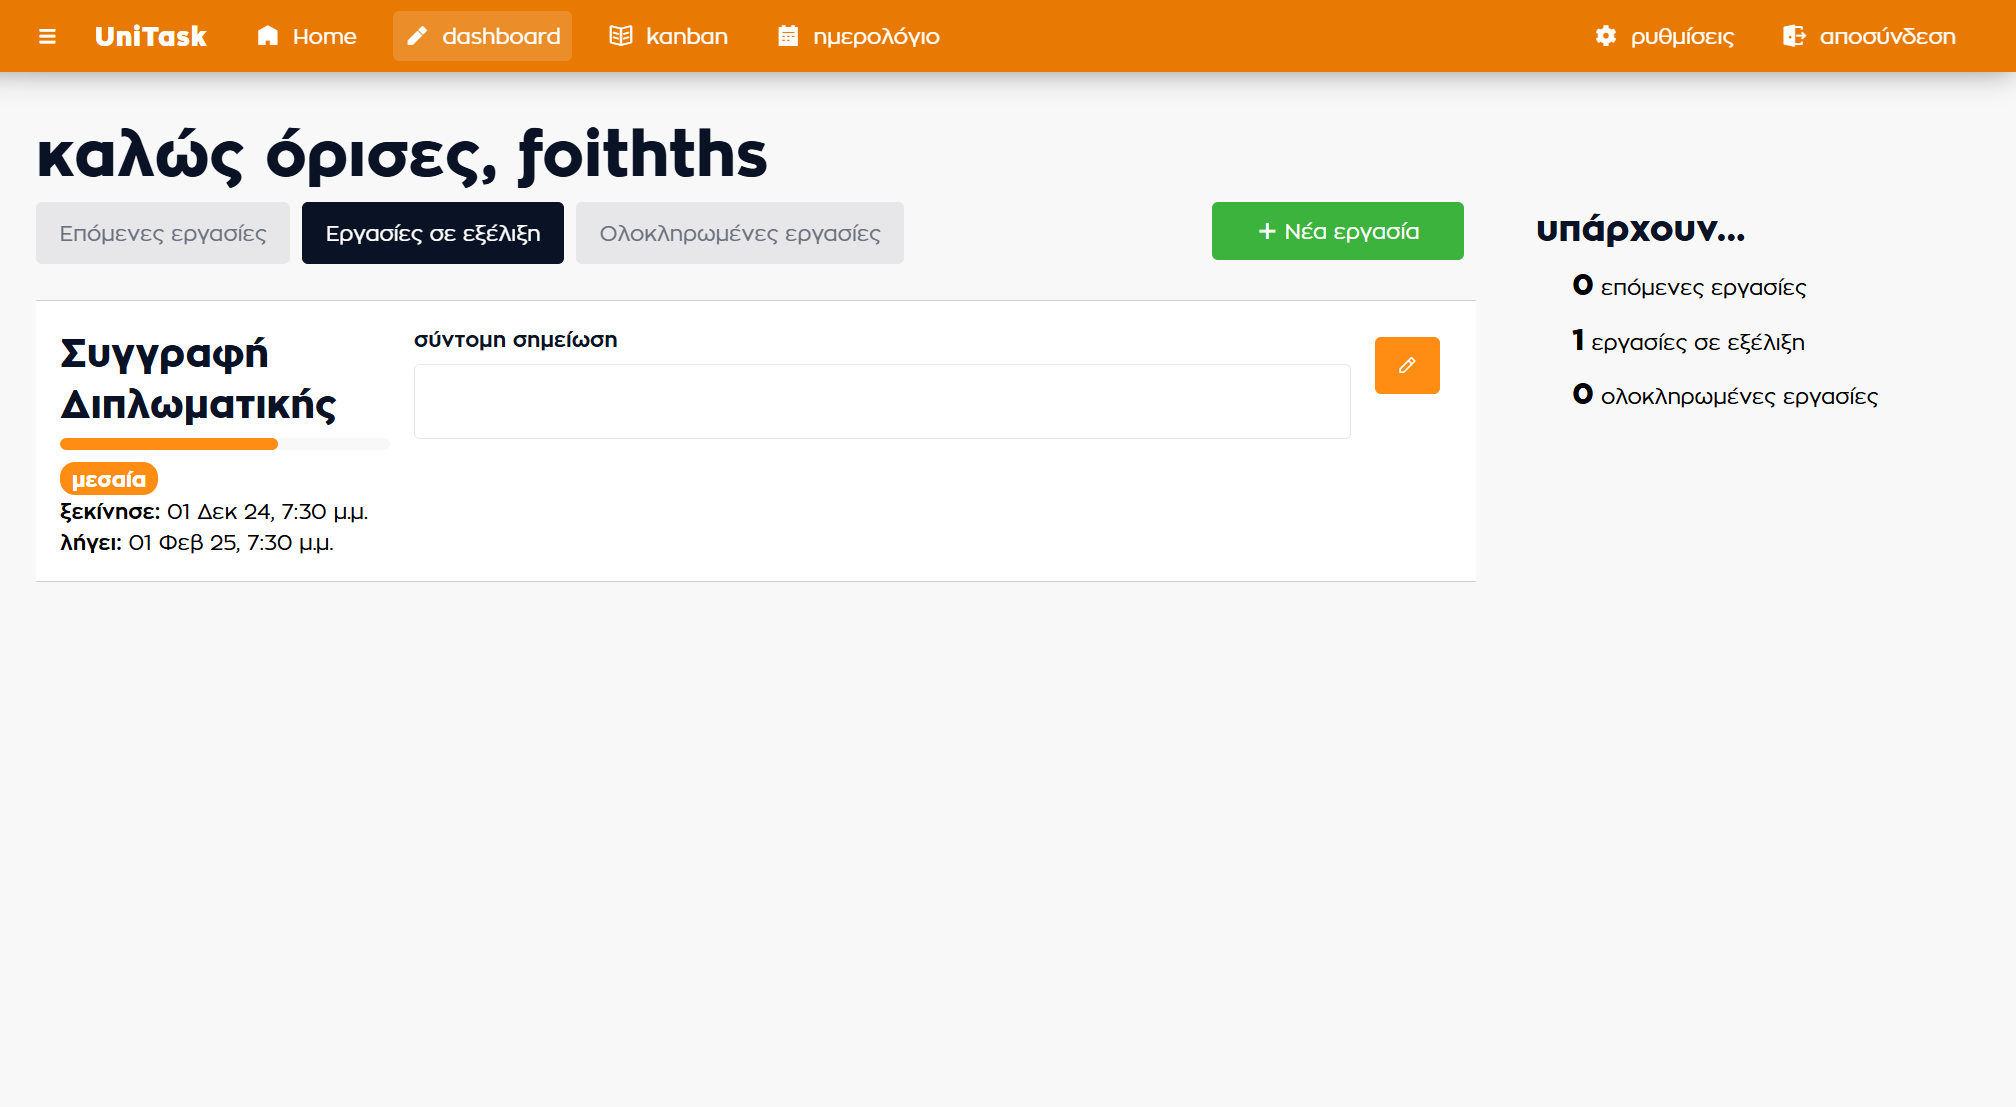
\includegraphics[trim={0 10cm 0 0}, clip, width=\textwidth]{UniTask/TaskDashboard_WithTask}
%            \caption{\centering Dashboard με δημιουργημένη εργασία}
%            \label{fig:unitask_TaskDashboard_WithTask}
%        \end{figure}
%
%        Στη σελίδα πλέον είναι δημιουργημένη η κάρτα με την πρώτη μας εργασία (σχήμα \ref{fig:unitask_TaskDashboard_WithTask}). Στο πλαίσιο {\Zona σύντομη σημείωση} μπορούμε να προσθέσουμε μια σύντομη περιγραφή της εργασίας, στα αριστερά εμφανίζεται ο τίτλος της εργασίας, μια μπάρα προόδου (progress bar) η οποία δυναμικά αυξάνεται όσο πλησιάζουμε στη λήξη της εργασίας, όπως επίσης η προτεραιότητα της εργασίας και οι ημερομηνίες και ώρες εκκίνησης και λήξης της εργασίας, ενώ στο δεξί μέρος της κάρτας εμφανίζονται το εικονίδιο για την επεξεργασία της εργασίας.
%
%        Ο τρόπος εμφάνισης των εργασιών στο dashboard λαμβάνει υπόψη του την προτεραιότητα τους και τον χρόνο λήξης τους. Έτσι μια εργασία με υψηλή προτεραιότητα θα εμφανίζεται ψηλότερα από μια εργασία με χαμηλή προτεραιότητα που δε λήγει σύντομα.
%
%        \begin{figure}[h!] \noindent \centering
%            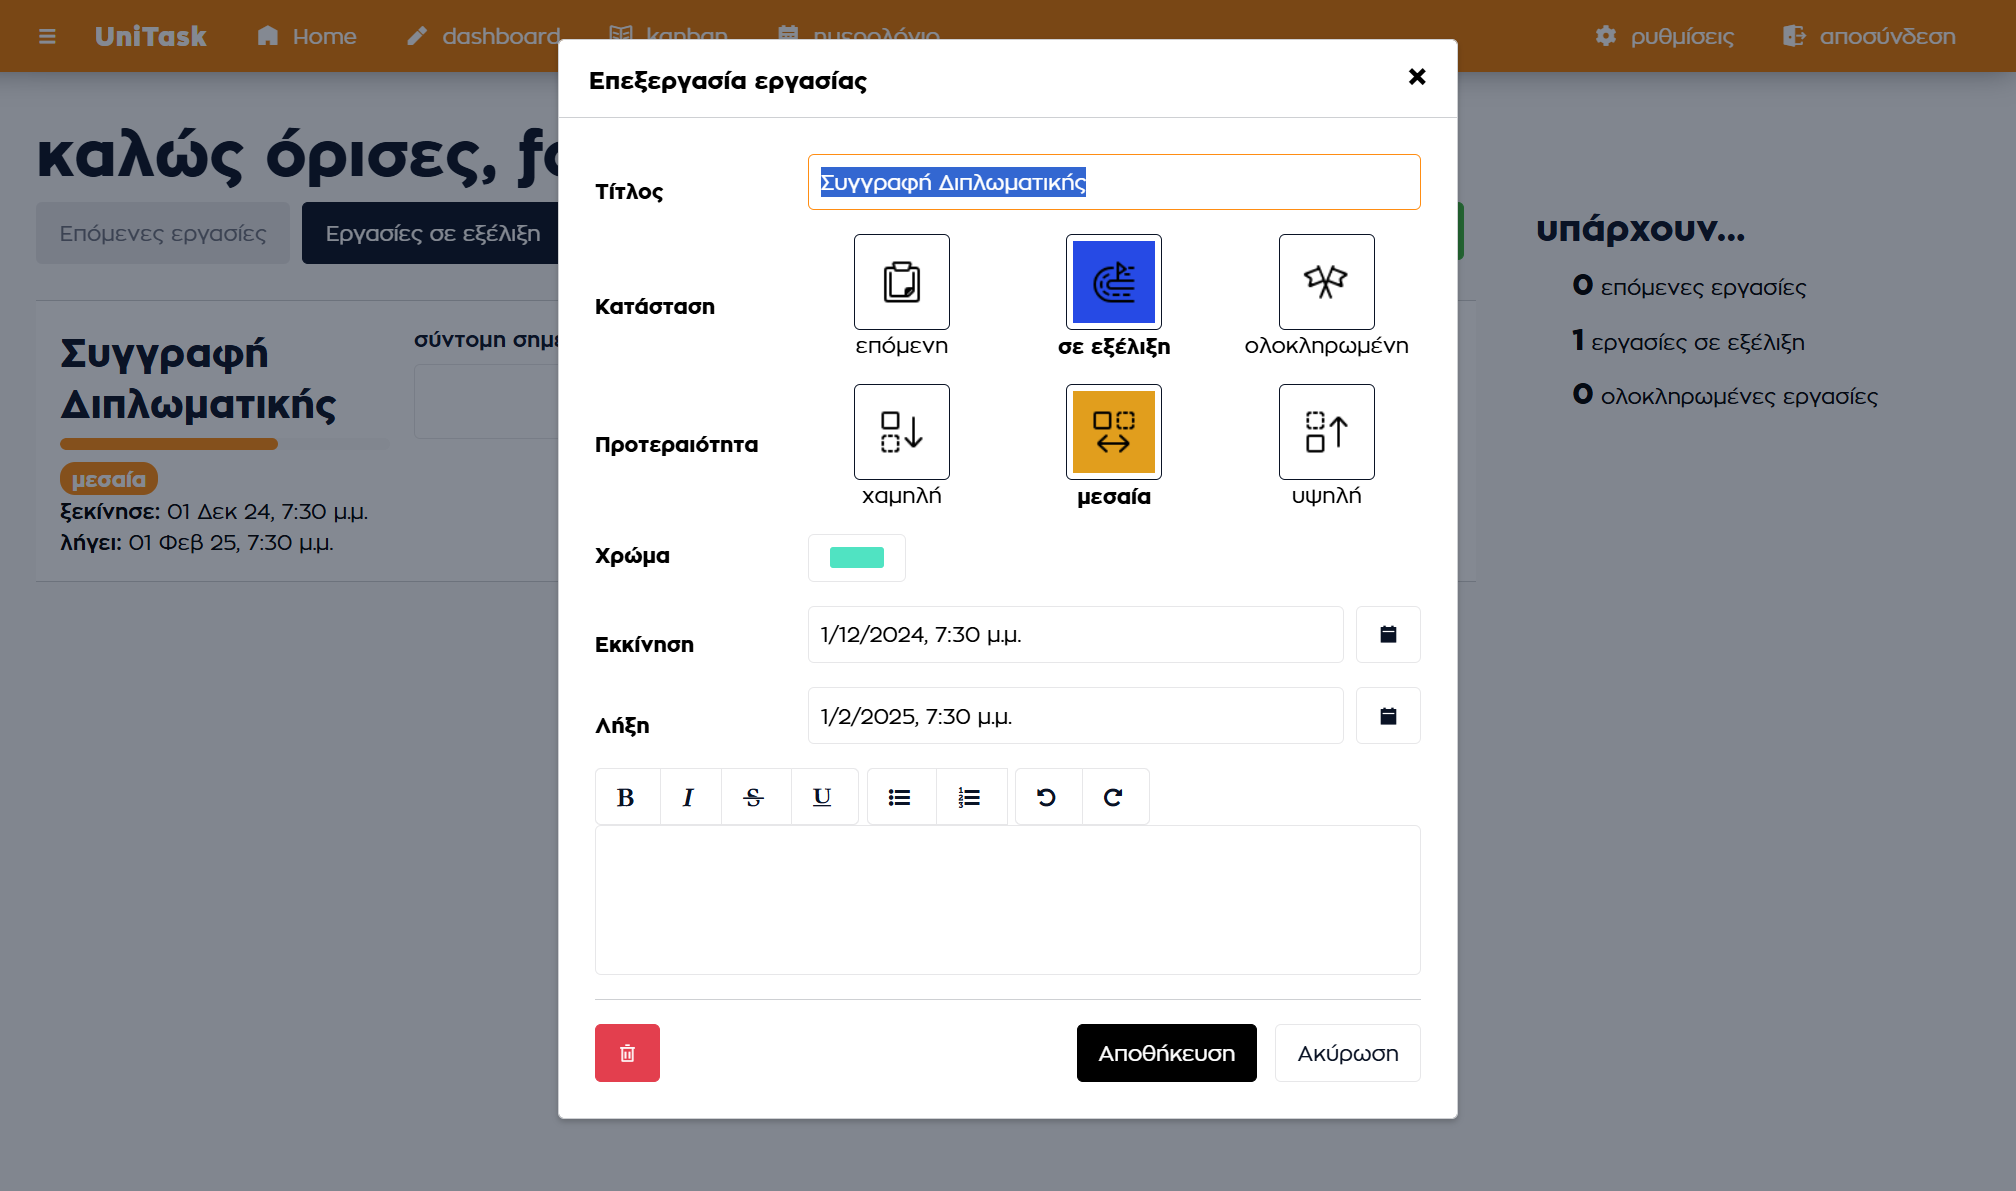
\includegraphics[width=\textwidth]{UniTask/EditTask}
%            \caption{\centering Επεξεργασία εργασίας}
%            \label{fig:unitask_EditTask}
%        \end{figure}
%
%        Πατώντας στο εικονίδιο επεξεργασίας, εμφανίζεται το popout παράθυρο του σχήματος \ref{fig:unitask_EditTask} όπου μπορούν να επεξεργαστούν τα στοιχεία της εργασίας μαζί με το πλαίσιο σύντομης σημείωσης. Το ίδιο παράθυρο περιλαμβάνει και το κουμπί διαγραφής της εργασίας.
%
%        \begin{figure}[h!] \noindent \centering
%            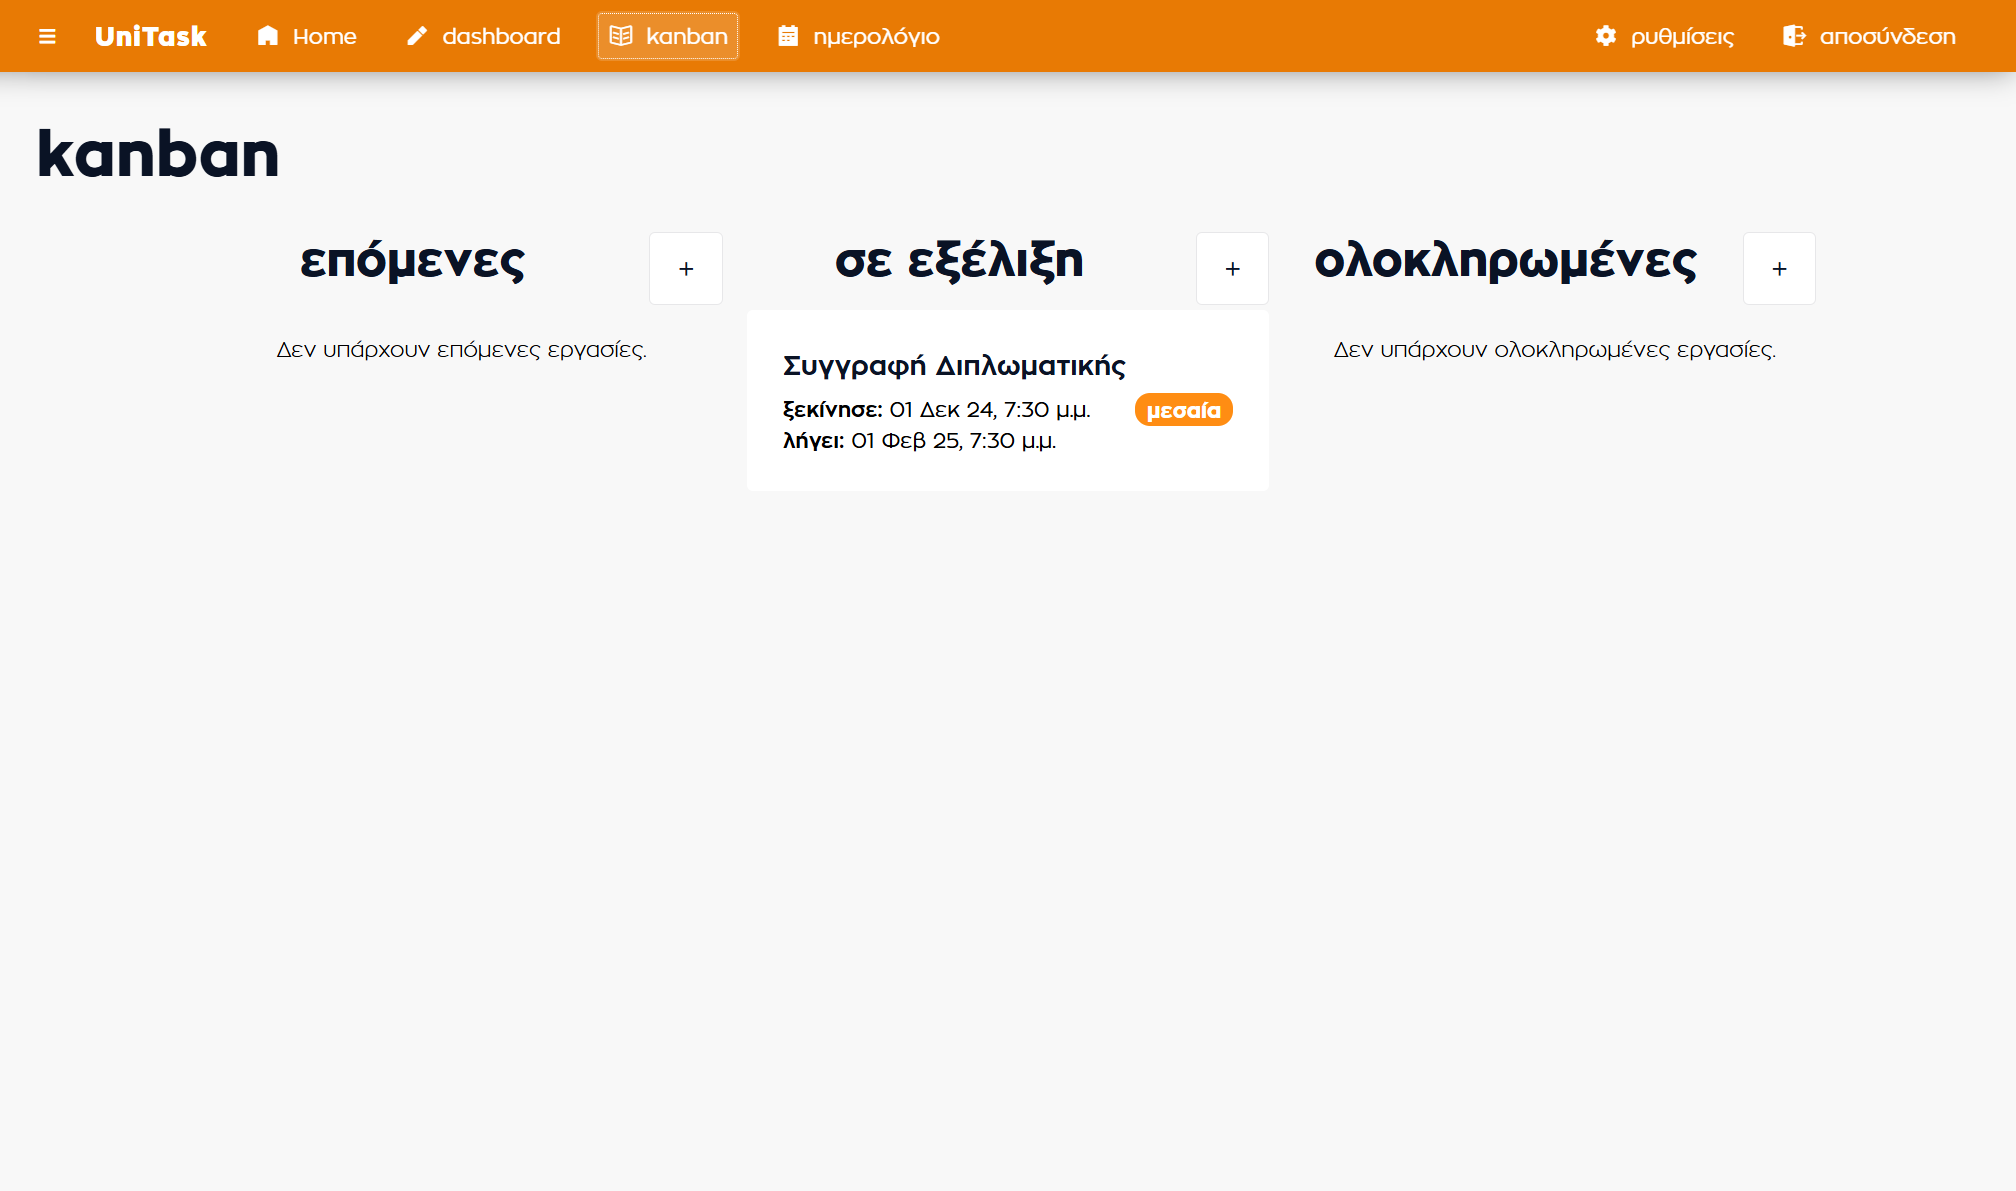
\includegraphics[trim={0 10cm 0 0}, clip, width=\textwidth]{UniTask/Kanban_WithTask}
%            \caption{\centering Σελίδα Kanban}
%            \label{fig:unitask_Kanban_WithTask}
%        \end{figure}
%
%        Η σελίδα {\ZonaSB Kanban} του σχήματος \ref{fig:unitask_Kanban_WithTask} εμφανίζει μια διαφορετική παρουσίαση στις εργασίες με τον τρόπο που έχει εξηγηθεί στην ενότητα \ref{subsec:Kanban}. Στον πίνακα Kanban οι εργασίες χωρίζονται σε τρεις κατηγορίες: τις εργασίες που έχουν ολοκληρωθεί, τις εργασίες που βρίσκονται σε εξέλιξη και τις εργασίες που έχουν σκοπό να πραγματοποιηθούν στο μέλλον. Κάθε στήλη περιλαμβάνει ένα κουμπί δημιουργίας νέας εργασίας που αυτόματα καθορίζει και την κατηγορία της.
%
%        Οι εργασίες εμφανίζονται σε κάρτες με τον τίτλο της εργασίας, την προτεραιότητα της, την ημερομηνία έναρξης και λήξης της, ενώ πατώντας πάνω στην κάρτα μιας εργασίας, εμφανίζεται το popout παράθυρο επεξεργασίας της εργασίας του σχήματος \ref{fig:unitask_EditTask}.
%
%        Στη σελίδα {\ZonaSB ημερολόγιο} (σχήμα \ref{fig:unitask_Calendar_WithTask}) εμφανίζεται ένα ημερολόγιο με τις εργασίες του χρήστη. Οι εργασίες εμφανίζονται στο ημερολόγιο με το χρώμα που έχει οριστεί στην επιλογή του χρήστη κατά τη δημιουργία της εργασίας, υπάρχουν προβολές ανά ημέρα, εβδομάδα ή μήνα ενώ εμφανίζεται και ένα σύντομο παράρτημα στα δεξιά με την λίστα των εργασιών.
%
%        \begin{figure}[h!] \noindent \centering
%            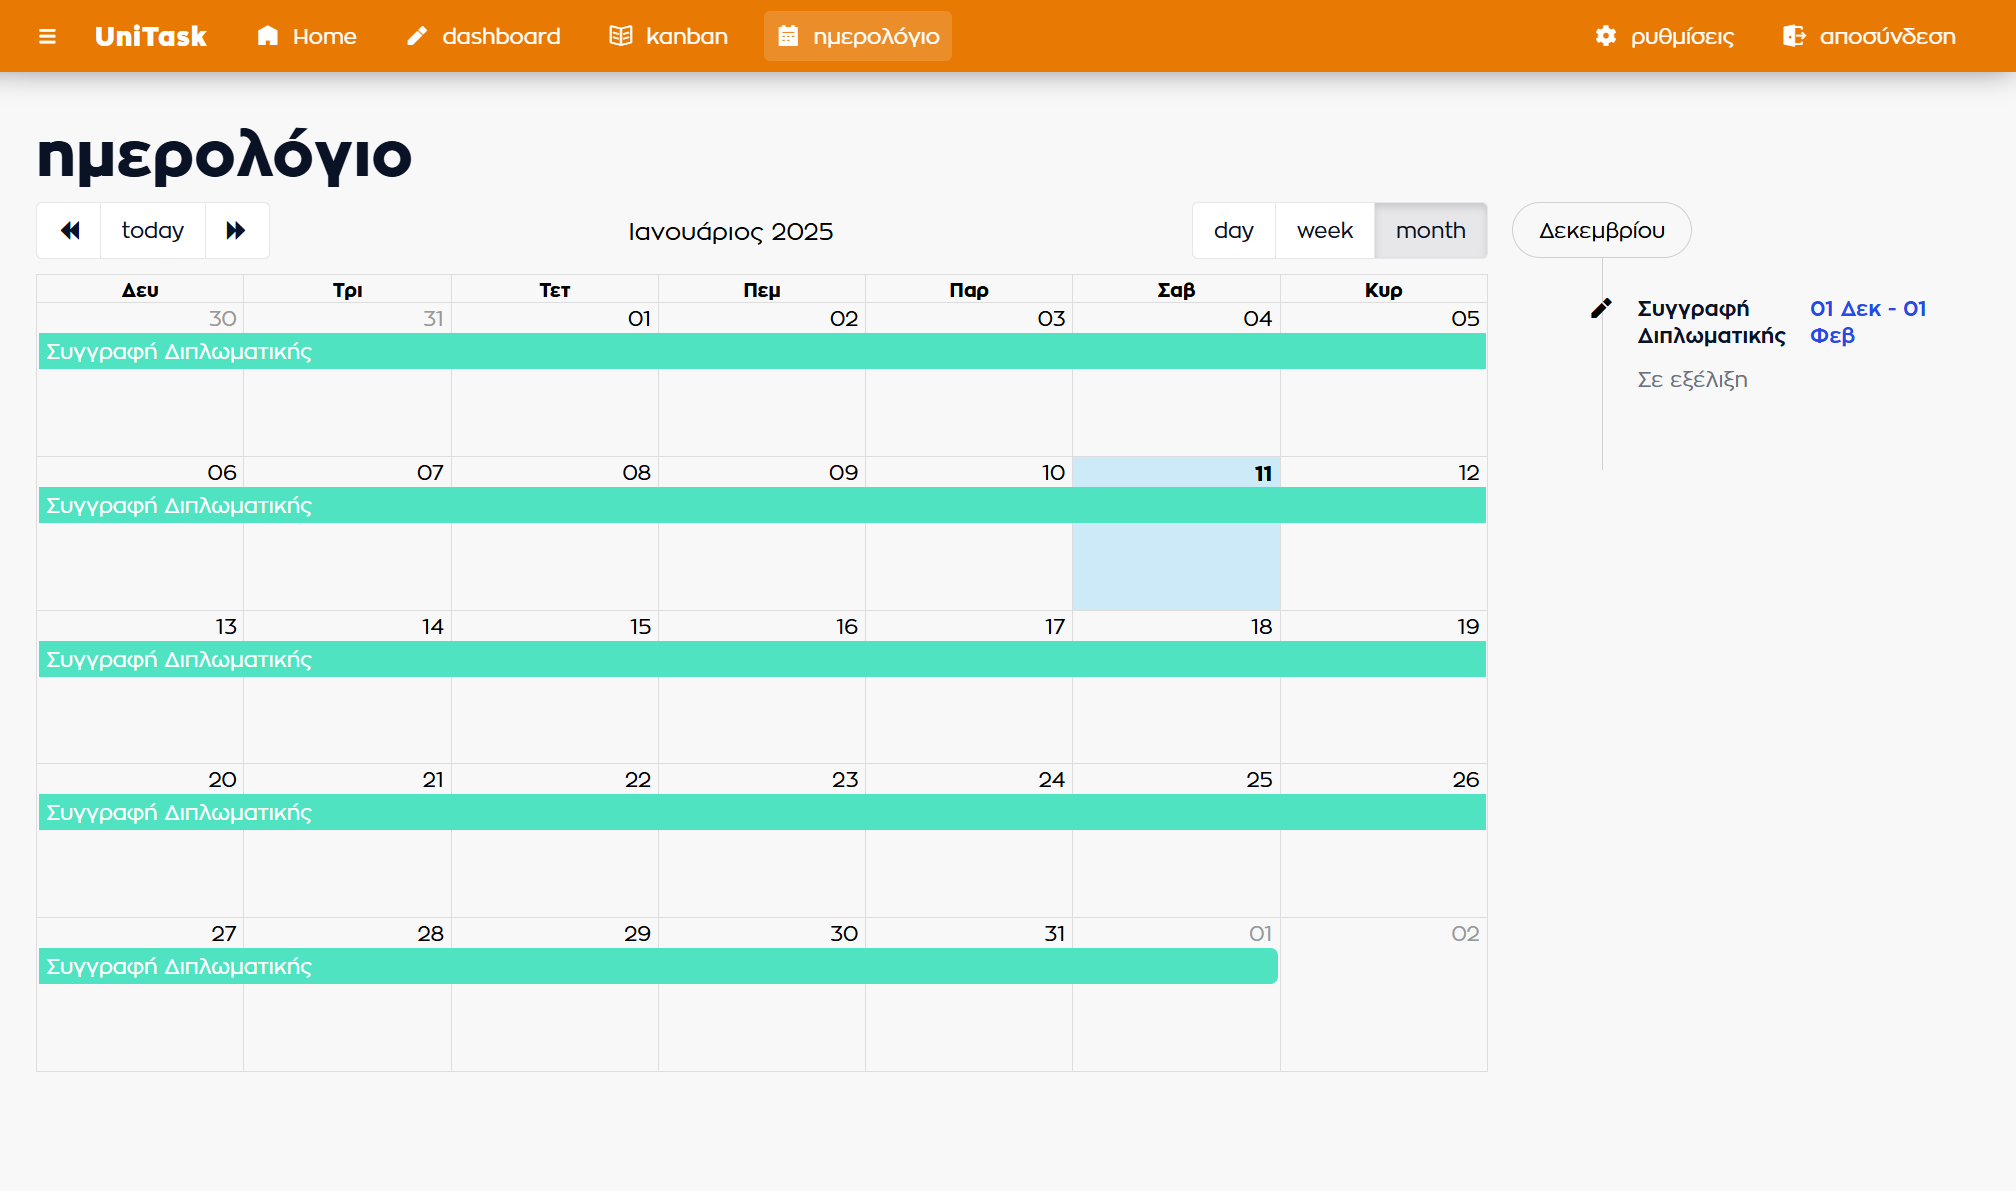
\includegraphics[width=\textwidth]{UniTask/Calendar_WithTask}
%            \caption{\centering Σελίδα Calendar}
%            \label{fig:unitask_Calendar_WithTask}
%        \end{figure}
%
%        Τέλος, στη σελίδα {\ZonaSB ρυθμίσεις} (σχήμα \ref{fig:unitask_Settings}) μπορούμε με ένα κουμπί να διαγράψουμε όλες τις εργασίες μας, ή να επιλέξουμε τη λειτουργία γρήγορης διαγραφής εργασιών. Αυτή η λειτουργία εισάγει ένα κουμπί διαγραφής στις κάρτες εργασιών στο dashboard, επιτρέποντας την άμεση διαγραφή των εργασιών που θέλουμε χωρίς να χρειάζεται να μεταβούμε στη σελίδα επεξεργασίας κάθε εργασίας (σχήμα \ref{fig:unitask_Dashboard_Kanban_Calendar_WithTasks}.1). Τέλος, παρέχεται η δυνατότητα αρχικοποίησης των εργασιών. Στην αρχικοποίηση διαγράφονται οι υπάρχουσες εργασίες του χρήστη και δημιουργούνται κάποιες προκαθορισμένες οι οποίες λειτουργούν ως ένα demo (σχήμα \ref{fig:unitask_Dashboard_Kanban_Calendar_WithTasks}).
%
%        \begin{figure}[h!] \noindent \centering
%            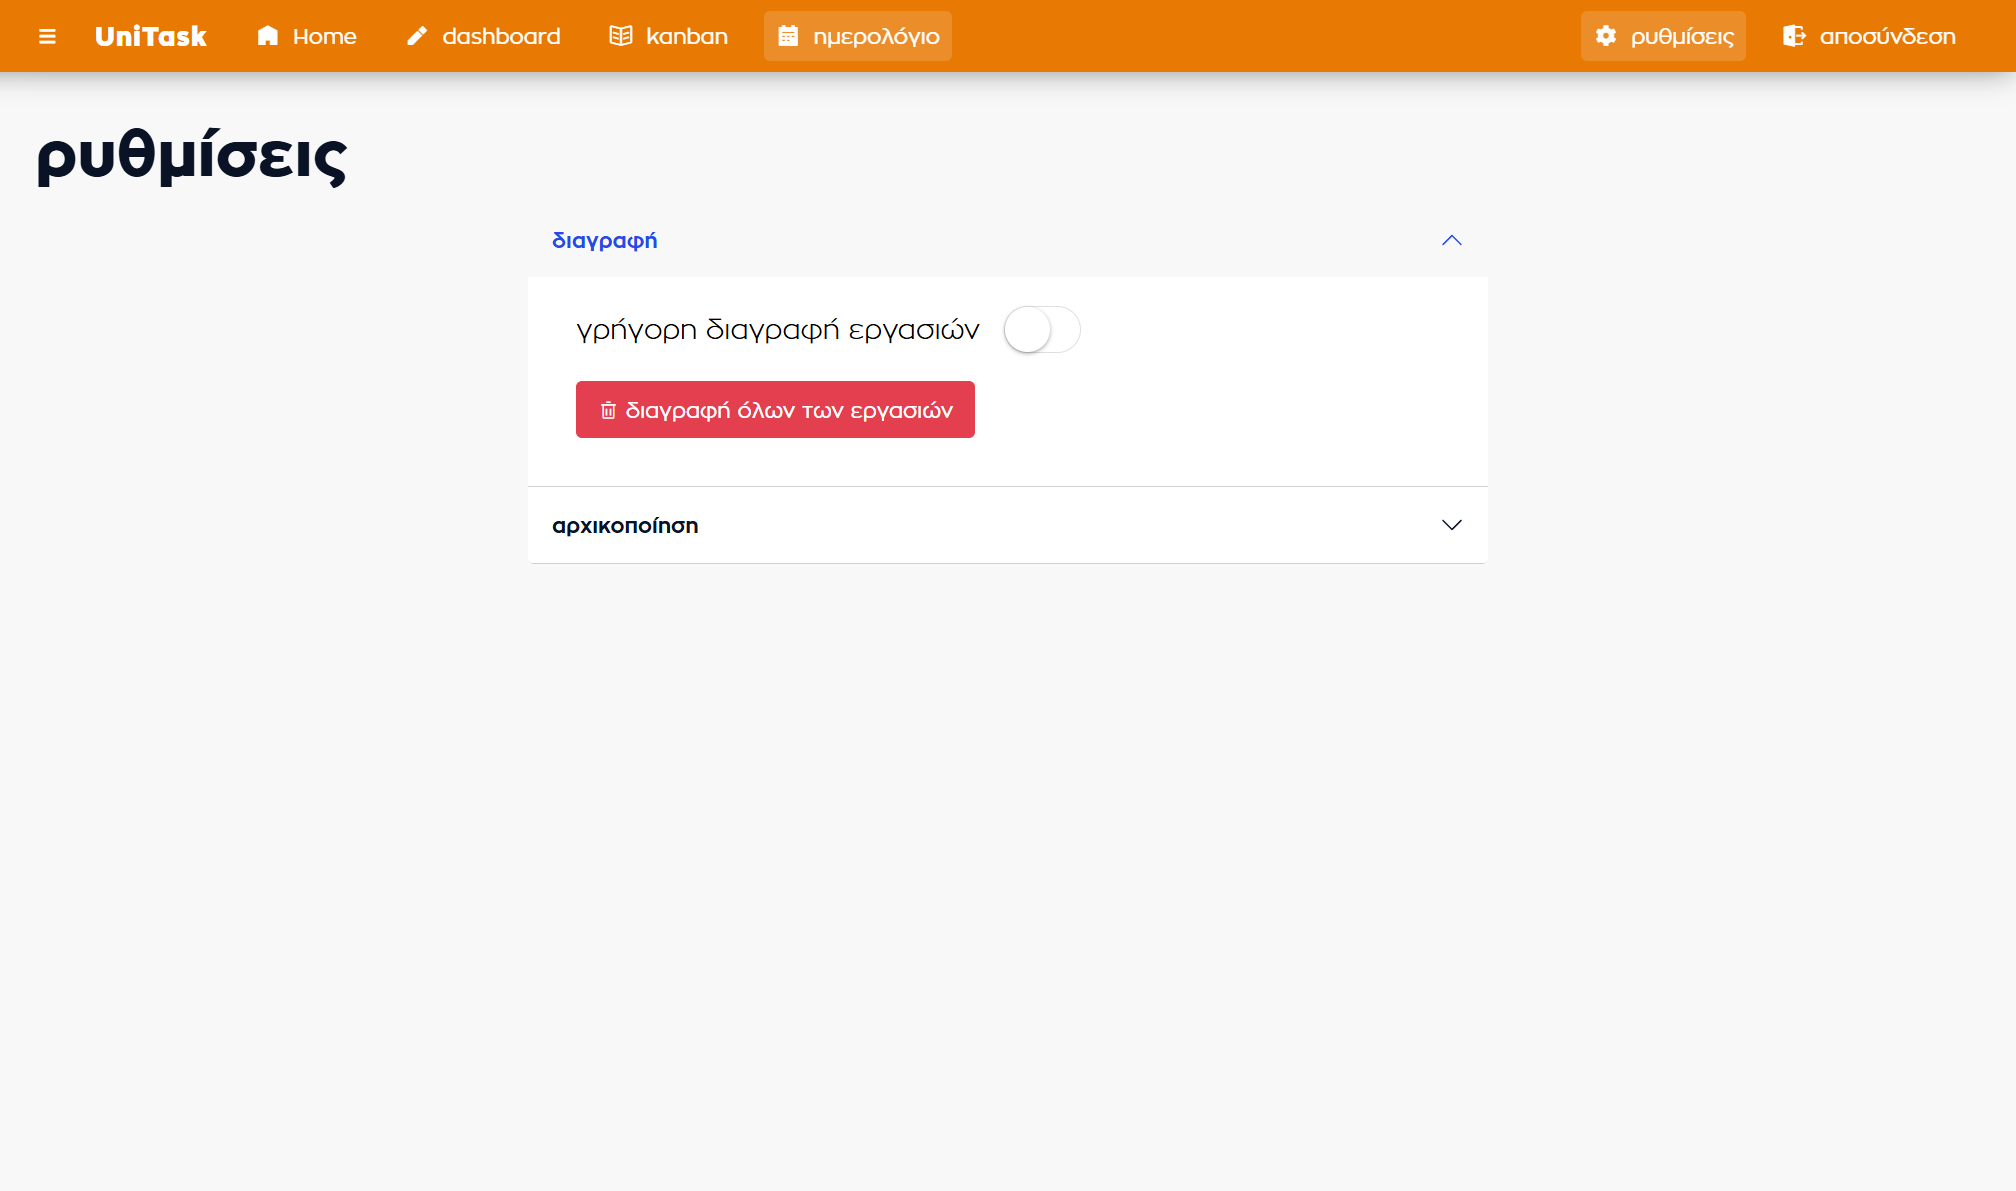
\includegraphics[trim={0 20cm 0 0}, clip, width=\textwidth]{UniTask/Settings_1}
%            
\includegraphics[width=\textwidth]{UniTask/Settings_2}
%            \caption{\centering Σελίδα ρυθμίσεων}
%            \label{fig:unitask_Settings}
%        \end{figure}
%
%        Σε κάθε ρύθμιση εμφανίζονται επιβεβαιωτικά popout μηνύματα προκειμένου να αποφευχθούν ακούσιες διαγραφές εργασιών (σχήμα \ref{fig:unitask_InitializationPopUp}).
%
%        \begin{figure}[h!] \noindent \centering
%            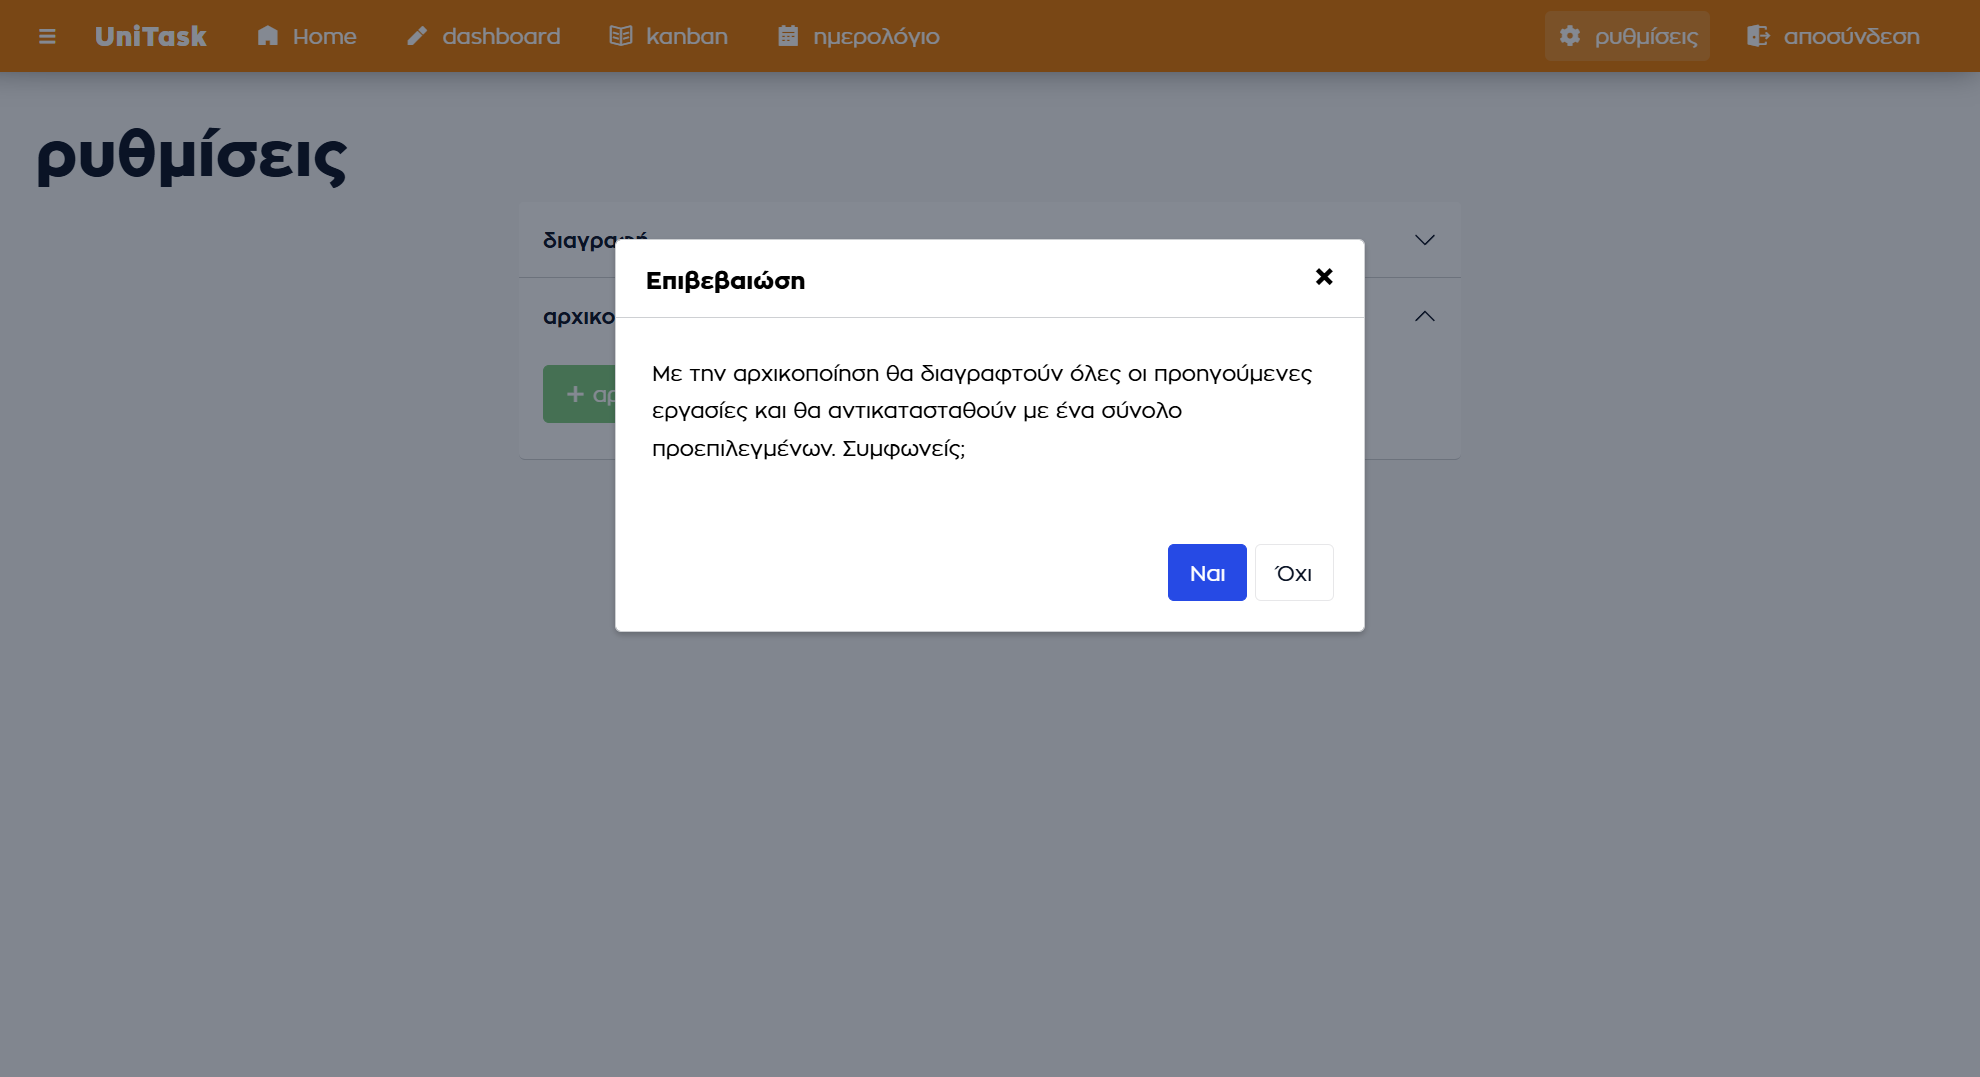
\includegraphics[trim={0 10cm 0 0}, clip, width=\textwidth]{UniTask/InitializationPopUp}
%            \caption{\centering Σελίδα ρυθμίσεων}
%            \label{fig:unitask_InitializationPopUp}
%        \end{figure}
%
%        \begin{figure}[p!] \noindent \centering
%            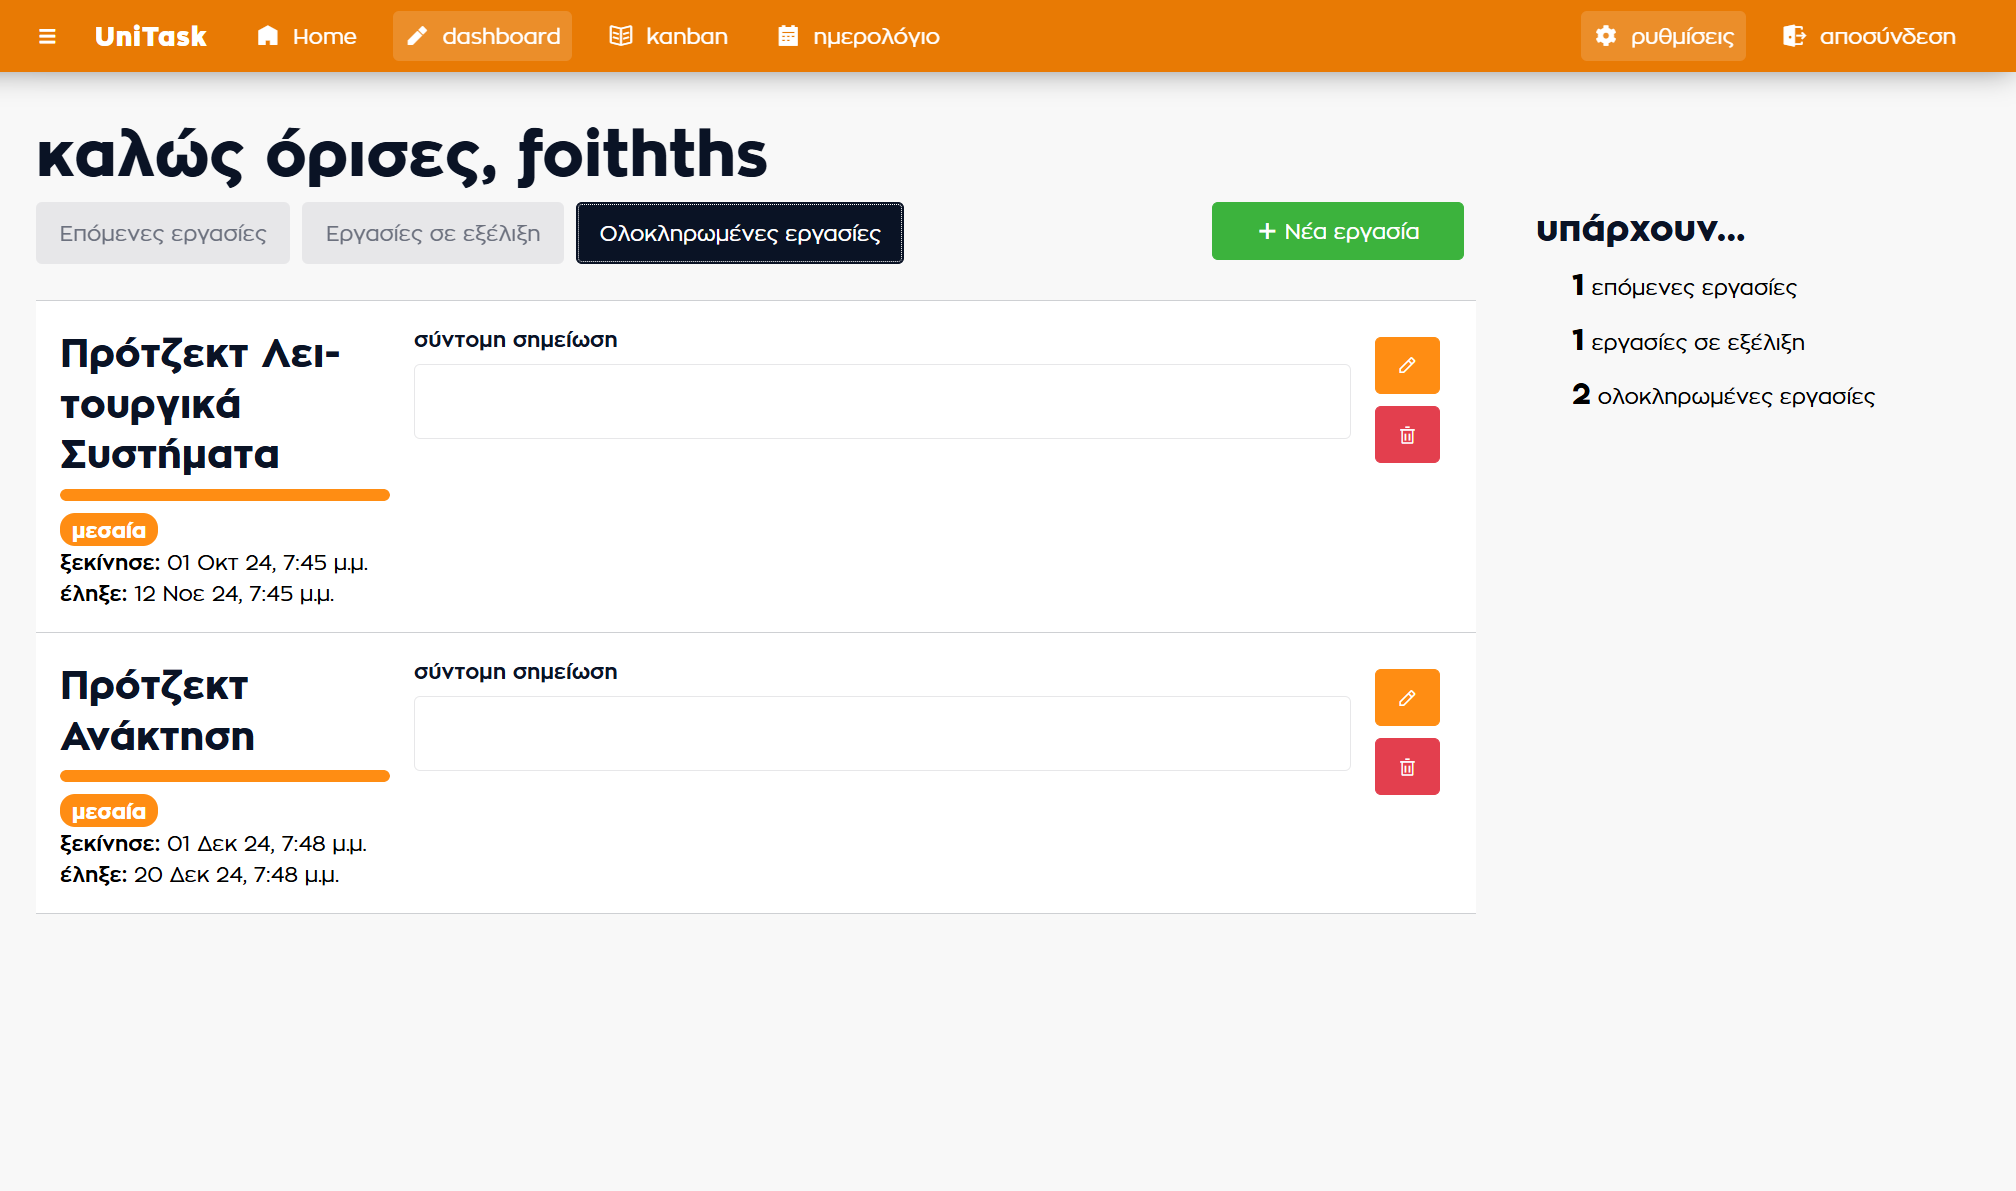
\includegraphics[trim={0 5cm 0 0}, clip, width=\textwidth]{UniTask/TaskDashboard_QuickDelete}
%            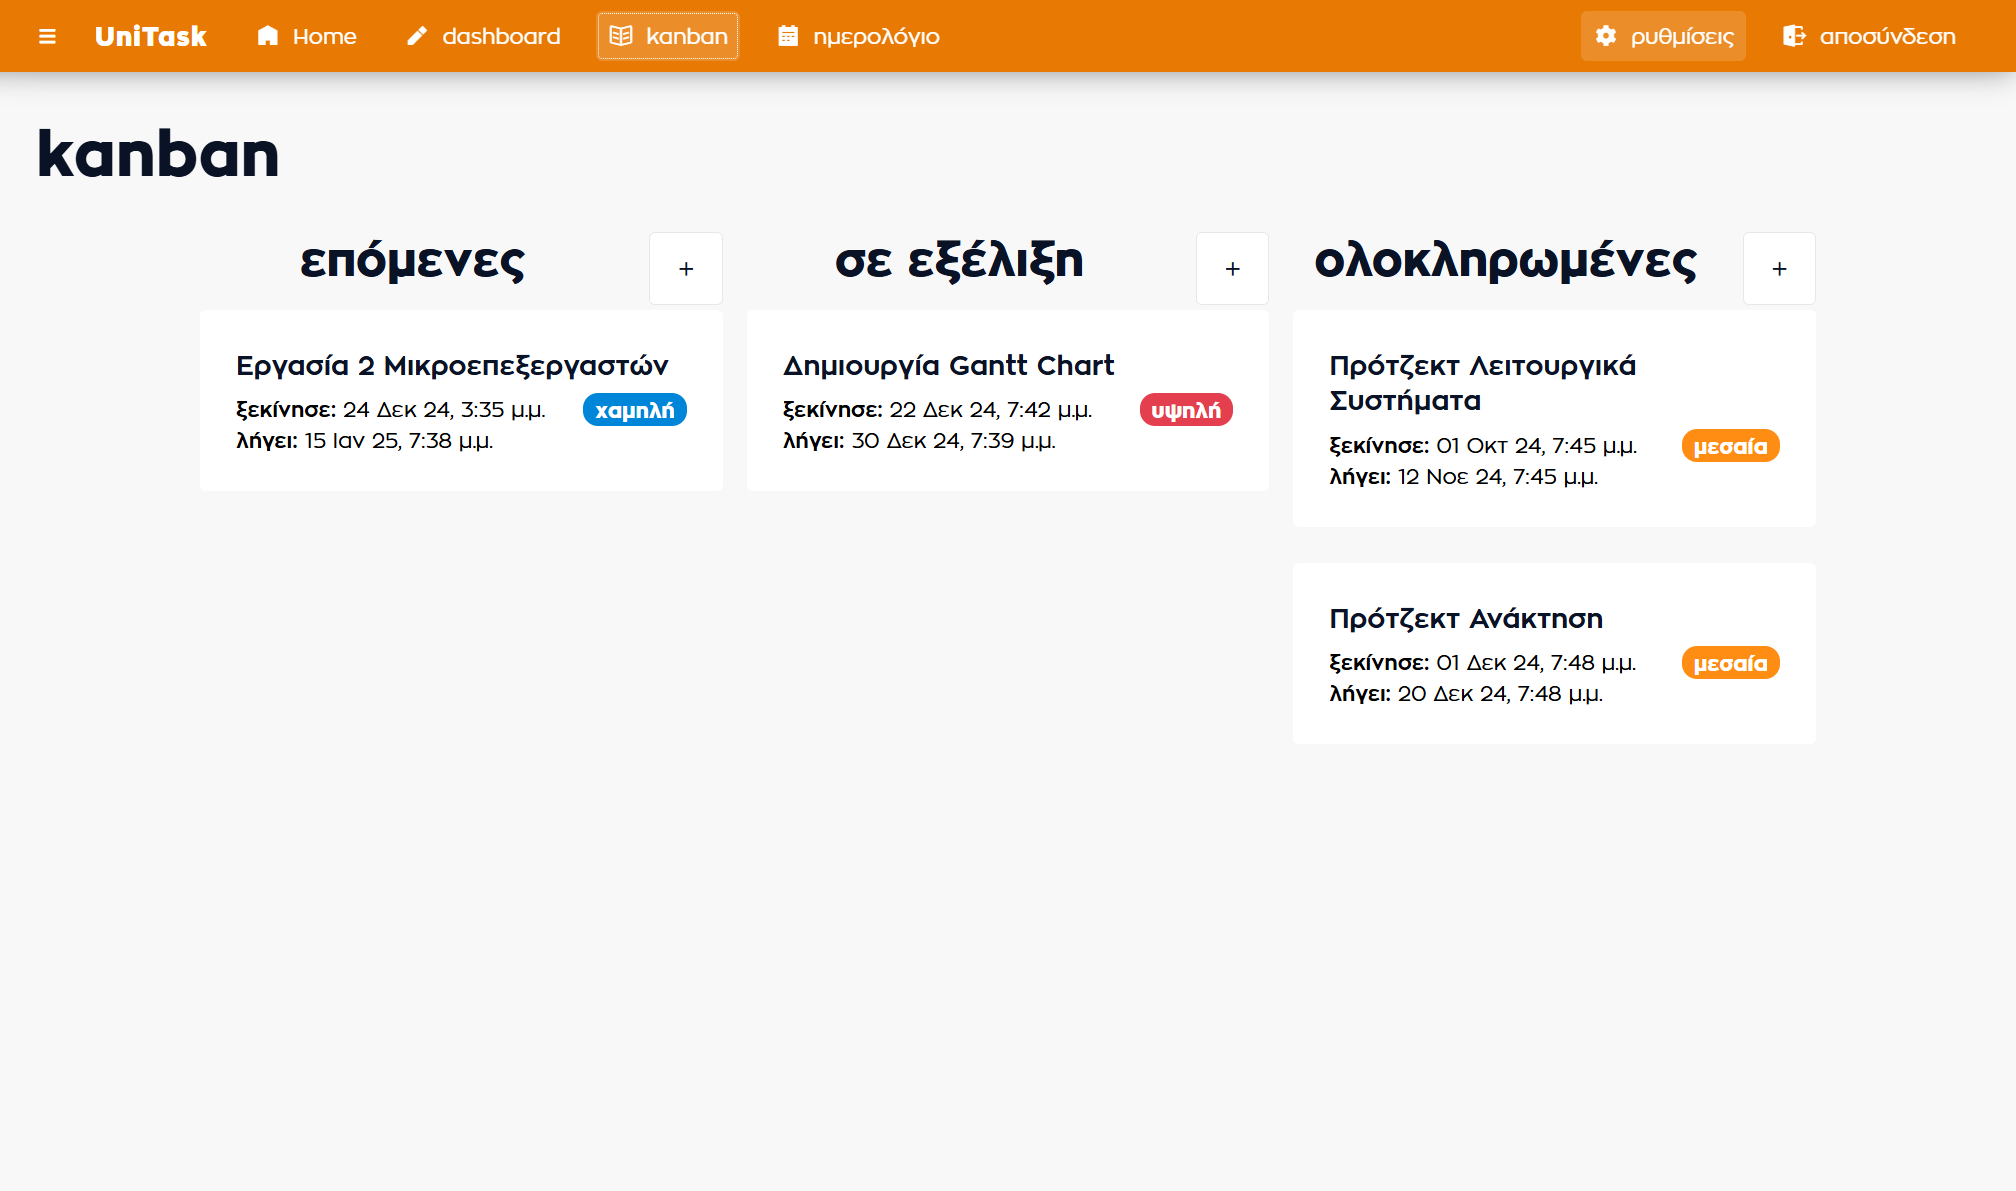
\includegraphics[trim={0 10cm 0 0}, clip, width=\textwidth]{UniTask/Kanban_WithTasks}
%            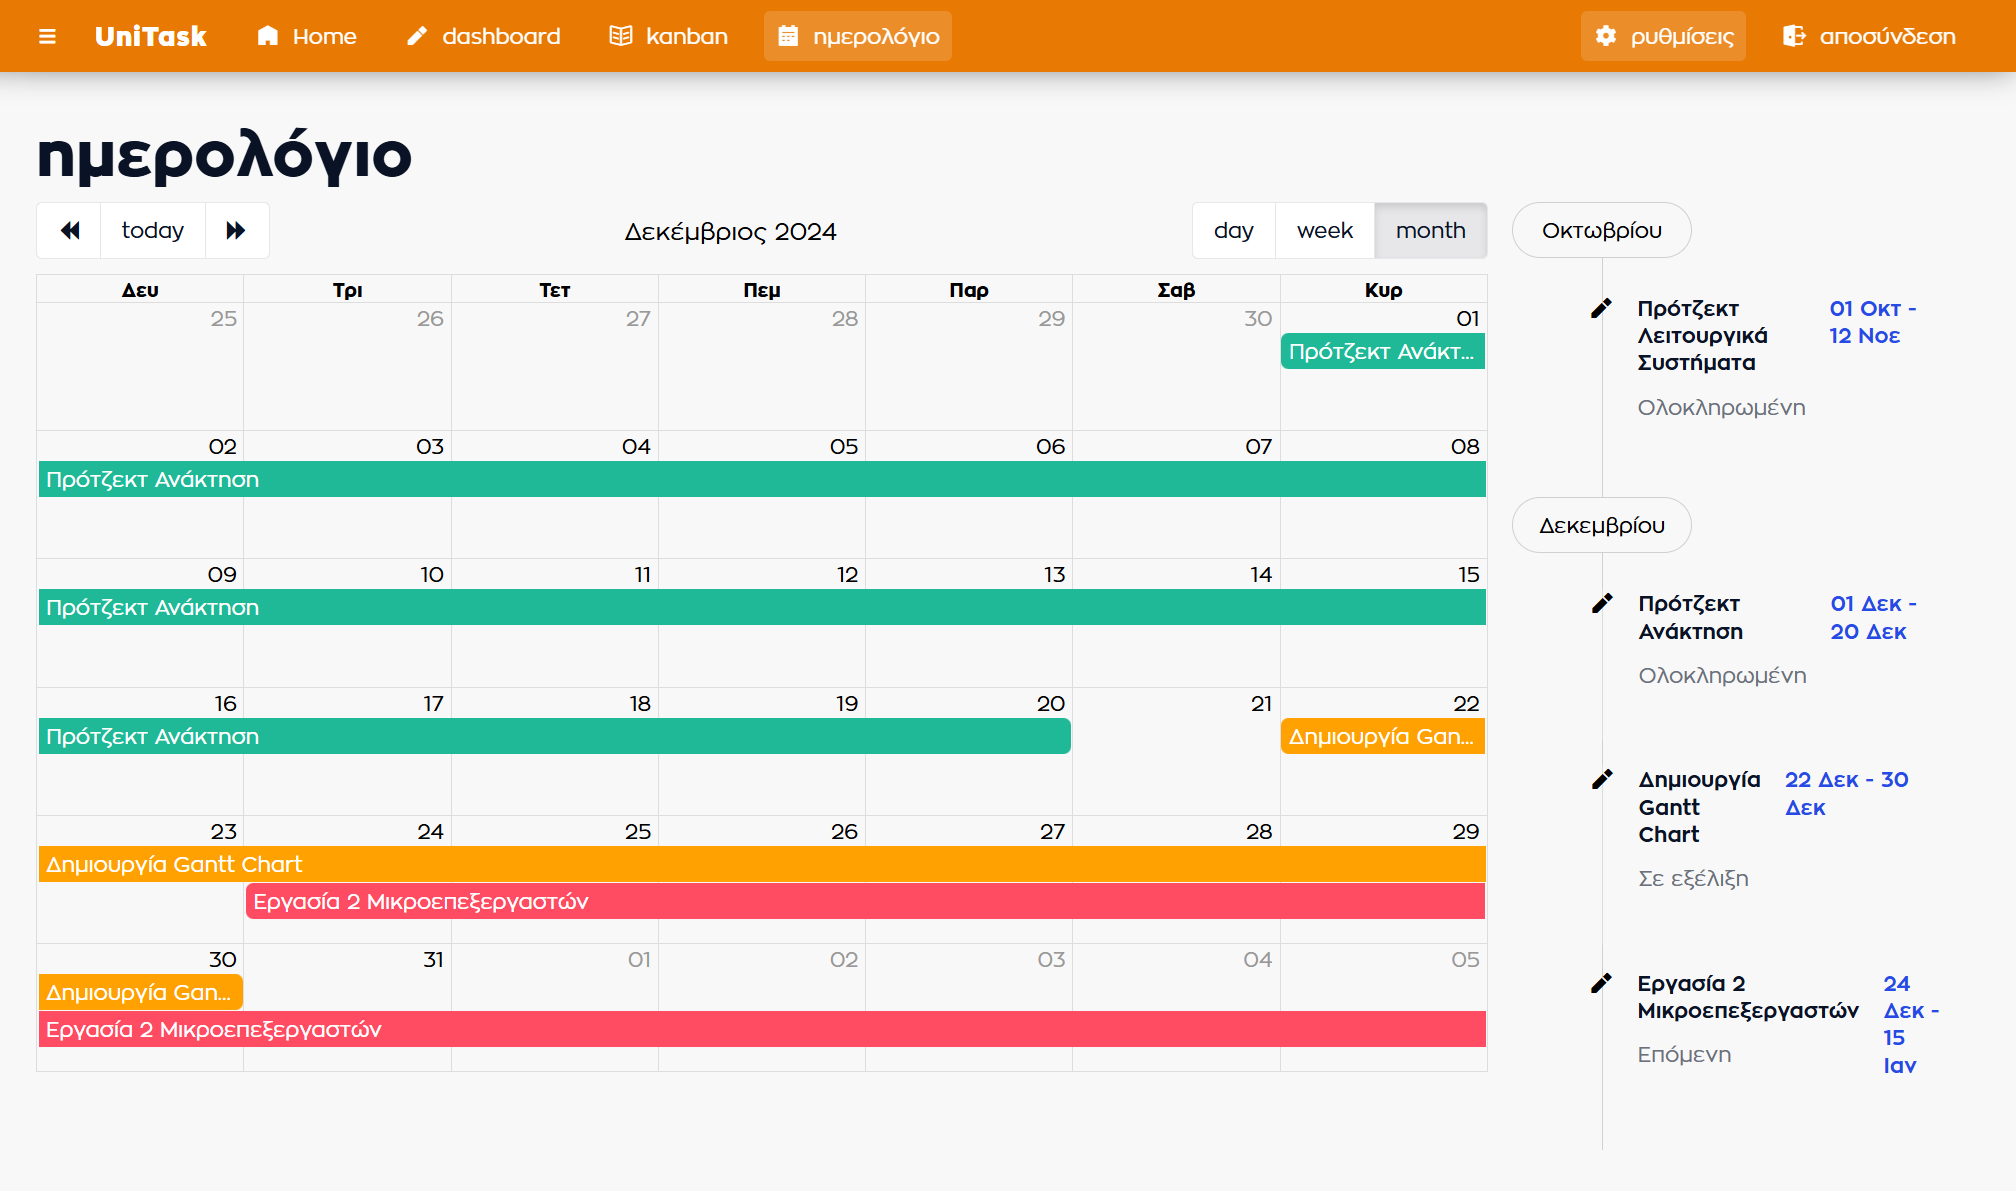
\includegraphics[width=\textwidth]{UniTask/Calendar_WithTasks}
%            \caption{\centering Οι σελίδες Dashboard, Kanban και Calendar μετά την αρχικοποίηση των εργασιών. Στο Dashboard φαίνεται η λειτουργία γρήγορης διαγραφής εργασιών.}
%            \label{fig:unitask_Dashboard_Kanban_Calendar_WithTasks}
%        \end{figure}

    \section{Δομή της εφαρμογής} \label{sec:unitask_mendix}
        Πέρα από τα προκατασκευασμένα modules του Mendix, η λειτουργικότητα της εφαρμογής έχει οργανωθεί σε τρία modules, το \texttt{Administrator}, το \texttt{TaskManager} και το \texttt{UniTask}.

        \subsection{Module \texttt{Administrator}}
            Το \texttt{Administrator} περιλαμβάνει τη λειτουργικότητα που αφορά τη διαχείριση των χρηστών της εφαρμογής. Όλες οι οντότητες του domain model, οι σελίδες και τα microflows του module έχουν δικαιώματα ανάγνωσης και εγγραφής από τον \texttt{Administrator} ρόλο, όπως ορίζεται στο \texttt{Security} της εφαρμογής.

            \subsubsection{Domain model του \texttt{Administrator}}
                \begin{center}
                    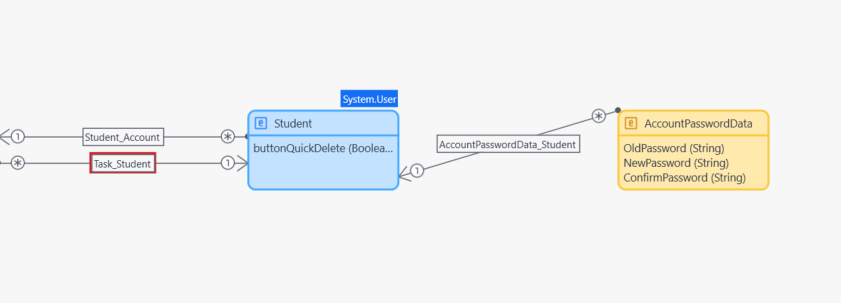
\includegraphics[width=0.9\textwidth]{UniTask_Mendix/Administrator_DomainModel}
                \end{center}

                Το domain model του \texttt{Administrator} περιλαμβάνει την οντότητα \texttt{Student} που κληρονομεί την οντότητα \texttt{System.User} του Mendix. Η οντότητα περιγράφει τον κάθε χρήστη της εφαρμογής και περιλαμβάνει την Boolean ιδιότητα \texttt{buttonQuickDelete} αρχικοποιημένη σε \texttt{False} η οποία χρησιμοποιείται για την ενεργοποίηση της λειτουργίας γρήγορης διαγραφής εργασιών. Η οντότητα \texttt{Student} συσχετίζεται με την οντότητα \texttt{Account} του \texttt{System.User} με σχέση 1-προς-1, η οντότητα \texttt{Task} του \texttt{TaskManager} με σχέση ένα-προς-πολλά (ένα Student συσχετίζεται με πολλά Tasks) και την οντότητα \texttt{AccountPasswordData} με σχέση 1-προς-πολλά (ένα Student συσχετίζεται με πολλά AccountPasswordData).

                Η οντότητα \texttt{AccountPasswordData} είναι μη-διατηρήσιμη οντότητα (δεν αποθηκεύεται στη βάση δεδομένων αλλά μόνο στη μνήμη) και περιλαμβάνει τις ιδιότητες \texttt{OldPassword}, \texttt{NewPassword} και \texttt{ConfirmPassword} και χρησιμοποιείται για την αλλαγή του κωδικού πρόσβασης του χρήστη.

            \subsubsection{Σελίδες του \texttt{Administrator}}
                Στο \texttt{Administrator} περιλαμβάνονται οι εξής σελίδες:

                \begin{figure}[H] \noindent
                    \paragraph{\texttt{Account\_Overview}}
                    \begin{center}
                        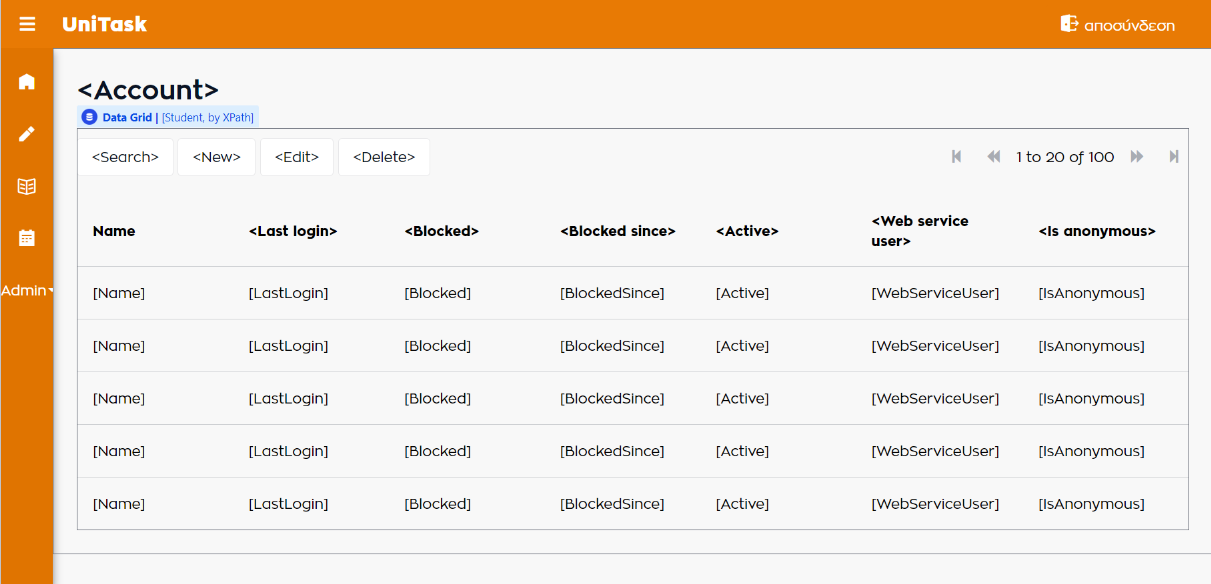
\includegraphics[width=0.9\textwidth]{UniTask_Mendix/Account_Overview}
                    \end{center}
                \end{figure}

                    Η σελίδα χρησιμοποιείται για τη διαχείριση των χρηστών της εφαρμογής από την πλευρά των διαχειριστών.

                    Χρησιμοποιείται το \texttt{UniTask\_SideBar} layout του \texttt{UniTaskDesignSystem} module. Το κύριο μέρος της σελίδας αποτελείται από ένα Data Grid με Data source την οντότητα \texttt{Student} και με στήλες τις ιδιότητες \texttt{Name}, \texttt{Last login}, \texttt{Blocked}, \texttt{Blocked since}, \texttt{Active}, \texttt{Web service user} και \texttt{Is anonymous}.

                \begin{figure}[H] \noindent
                    \paragraph{\texttt{Account\_New}}
                    \begin{center}
                        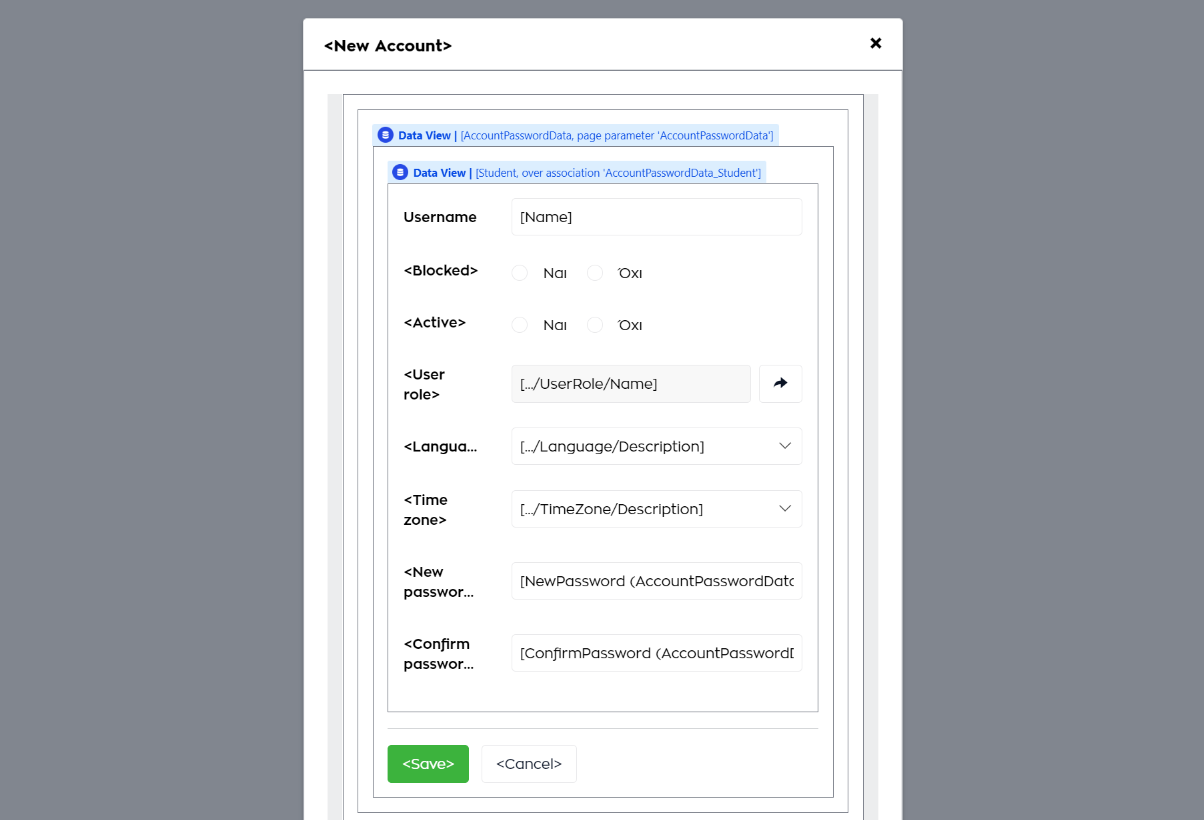
\includegraphics[width=0.9\textwidth]{UniTask_Mendix/Account_New}
                    \end{center}
                \end{figure}

                    Η σελίδα χρησιμοποιείται για τη δημιουργία νέων χρηστών της εφαρμογής.

                    Χρησιμοποιείται το \texttt{PopupLayout} layout του \texttt{Atlas\_Core} module. Η σελίδα περιλαμβάνει δύο Parameters, το \texttt{Student} και \texttt{AccountPasswordData} του module \linebreak \texttt{Administrator}. Η σελίδα αποτελείται από δύο εμφωλευμένα Data Views, το εξωτερικό έχει ως Data source το \texttt{AccountPasswordData}, ενώ το εσωτερικό έχει ως Data source τη συσχέτιση του \texttt{AccountPasswordData} με το \texttt{Student}. Η χρήση του \texttt{AccountPasswordData} είναι απαραίτητη καθώς η δημιουργία ενός νέου χρήστη χρειάζεται την αποθήκευση του κωδικού πρόσβασής του.

                    Στο εσωτερικό Data View περιλαμβάνει Text Boxes, Radio Buttons και Input \linebreak Reference Set Selectors όπου εισάγονται τιμές για τα \texttt{Username}, \texttt{Blocked}, \texttt{Active}, \texttt{User role}, \texttt{Language}, \texttt{Time zone}, \texttt{New password} και \texttt{Confirm password}. Έχει σημασία να σημειωθεί πως οι ιδιότητες (γνωρίσματα) που αποθηκεύουμε στην πραγματικότητα δεν είναι ιδιότητες του \texttt{Student} αλλά του \texttt{System.User} του οποίου αποτελεί παιδί. Το Input Reference Set Selector χρησιμοποιείται για την επιλογή του \texttt{UserRole}, που αποτελεί διαφορετική σελίδα που θα αναλυθεί στη συνέχεια.

                    Τέλος, περιλαμβάνεται κουμπί για την αποθήκευση, το οποίο καλεί το microflow \texttt{ACT\_Account\_Save} του \texttt{Administrator} για την αποθήκευση των τιμών, και κουμπί για την ακύρωση της διαδικασίας.

                \begin{figure}[H] \noindent
                    \paragraph{\texttt{Account\_Edit}}
                    \begin{center}
                        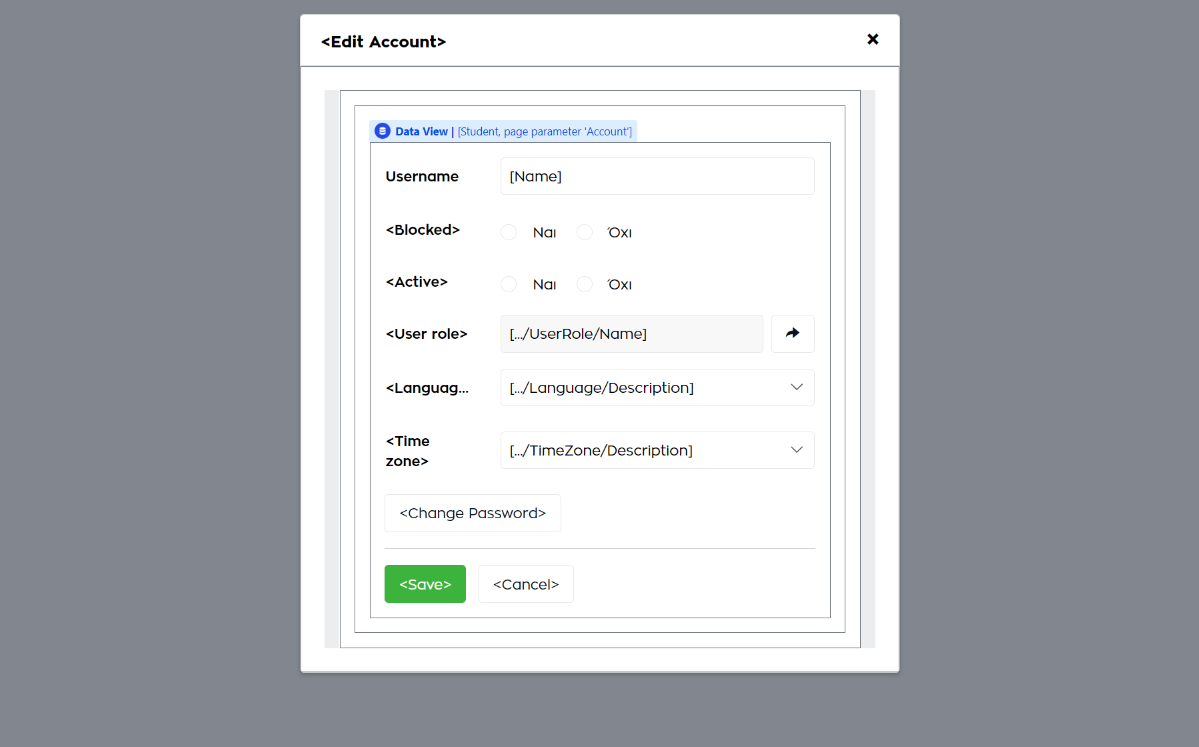
\includegraphics[width=0.9\textwidth]{UniTask_Mendix/Account_Edit}
                    \end{center}
                \end{figure}

                    Η σελίδα χρησιμοποιείται για την επεξεργασία υπαρχόντων χρηστών της εφαρμογής.

                    Χρησιμοποιείται το \texttt{PopupLayout}. Η σελίδα περιλαμβάνει το Parameter \texttt{Student}. Η σελίδα αποτελείται από ένα Data View με Data source το \texttt{Student} με παρόμοια Text Boxes και Radio Buttons όπως και το \texttt{Account\_New}. Επίσης, περιλαμβάνεται το κουμπί που καλεί το microflow \texttt{ACT\_Password\_Change} για την αλλαγή κωδικού.

                    Τέλος, περιλαμβάνεται κουμπί για την αποθήκευση και κουμπί για την ακύρωση της διαδικασίας. Τα κουμπιά καλούν προεπιλεγμένες ενέργειες του Mendix.

                \begin{figure}[H] \noindent
                    \paragraph{\texttt{Change\_Password}}
                    \begin{center}
                        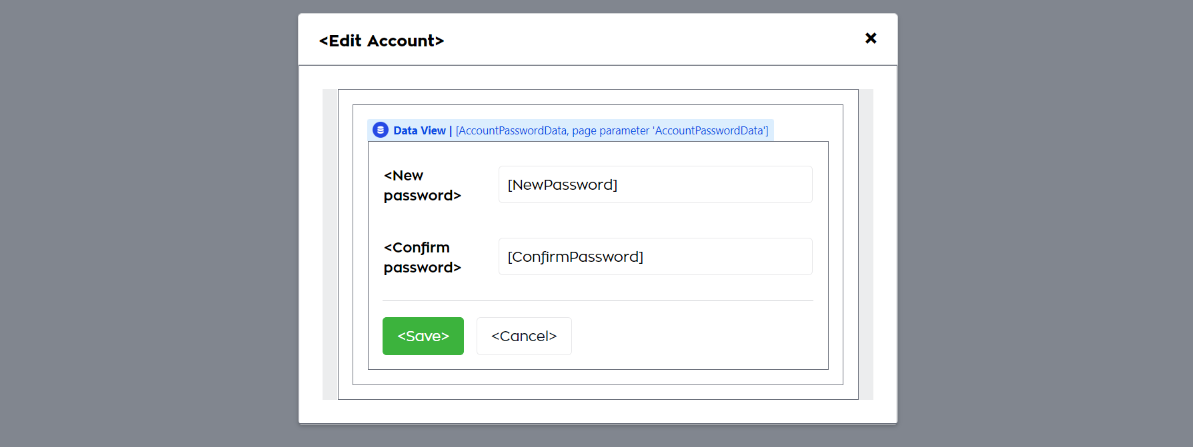
\includegraphics[width=0.9\textwidth]{UniTask_Mendix/Change_Password}
                    \end{center}
                \end{figure}

                    Η σελίδα χρησιμοποιείται για την αλλαγή του κωδικού πρόσβασης υπάρχοντος χρήστη.

                    Χρησιμοποιείται το \texttt{PopupLayout}. Η σελίδα περιλαμβάνει το Parameter \linebreak \texttt{AccountPasswordData}, ένα Data View με Data source το \texttt{Student} με τα απαραίτητα Text Boxes για την αλλαγή των τιμών. Τέλος, περιλαμβάνεται κουμπί για την αποθήκευση που καλεί το microflow \texttt{ChangePassword} του \texttt{Administrator} και κουμπί για την ακύρωση της διαδικασίας.

                \begin{figure}[H] \noindent
                    \paragraph{\texttt{UserRole\_Select}}
                    \begin{center}
                        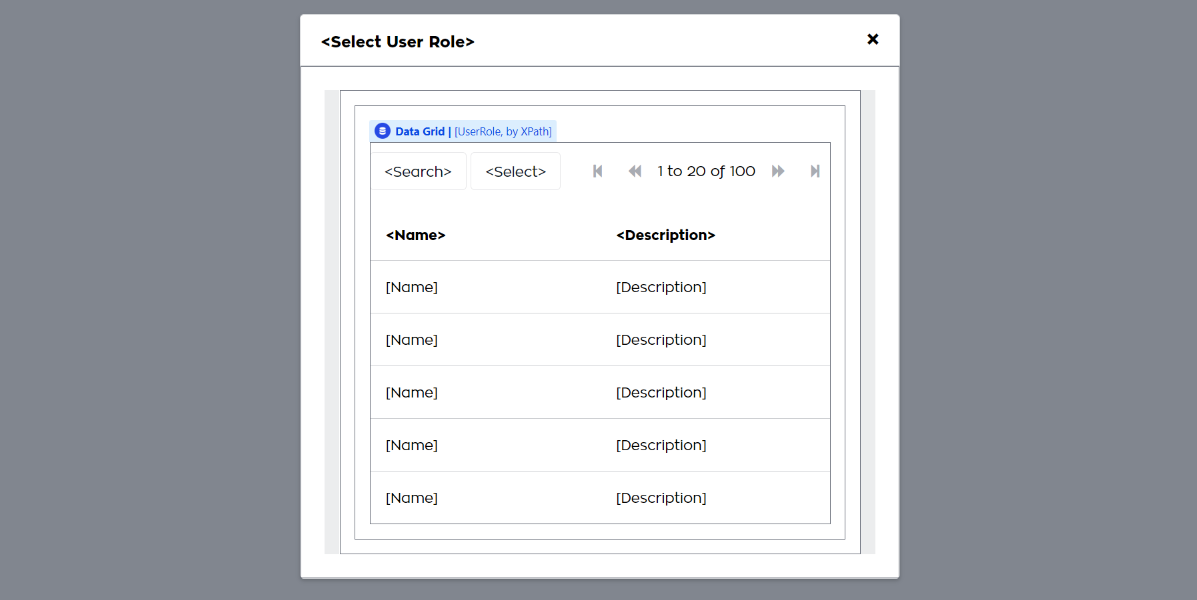
\includegraphics[width=0.9\textwidth]{UniTask_Mendix/UserRole_Select}
                    \end{center}
                \end{figure}

                    Η σελίδα χρησιμοποιείται για την επιλογή του ρόλου του χρήστη κατά τη δημιουργία νέου χρήστη.

                    Χρησιμοποιείται το \texttt{PopupLayout}. Η σελίδα αποτελείται από ένα Data Grid με Data source το \texttt{UserRole} του \texttt{System}.

            \subsubsection{Microflows του \texttt{Administrator}}
                Στο \texttt{Administrator} περιλαμβάνονται τα εξής microflows:

                \begin{figure}[H] \noindent
                    \paragraph{\texttt{VAL\_Account}}
                    \begin{center}
                        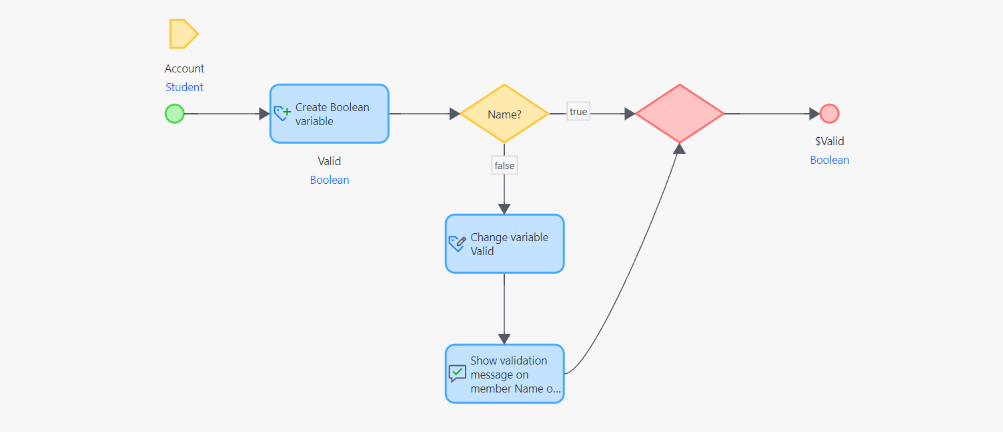
\includegraphics[width=0.9\textwidth]{UniTask_Mendix/VAL_Account}
                    \end{center}
                \end{figure}

                    To microflow καλείται από το microflow \texttt{ACT\_Account\_Save} για να επικυρώσει το λογαριασμό του χρήστη πριν αποθηκευτούν οι τιμές του.\footnote{Το πρόθεμα \texttt{VAL} χρησιμοποιείται στην ονομασία των microflows για να δηλώσει επικύρωση (validation).}

                    Αρχικά δημιουργείται μια boolean μεταβλητή \texttt{Valid} με αρχική τιμή \texttt{True} η οποία θα επιστραφεί από το microflow. Στη συνέχεια ελέγχεται αν για το αντικείμενο \texttt{Account} τύπου \texttt{Student} ισχύει η συνθήκη (\verb|trim($Account/Name) != ''|). Η έκφραση στη συνθήκη αφού καθαρίσει τα κενά (whitespaces) από το \texttt{Name} του \texttt{Account}, ελέγχει αν είναι διαφορετικό από το κενό string. Αν η συνθήκη δεν ισχύει, τότε η μεταβλητή \texttt{Valid} γίνεται \texttt{False}, η οποία επιστρέφεται μαζί με ένα popout μήνυμα. Αν η συνθήκη ισχύει, δηλαδή αν υπάρχει όνομα, τότε επιστρέφεται \texttt{True}.

                \begin{figure}[H] \noindent
                    \paragraph{\texttt{ACT\_Account\_New}}
                    \begin{center}
                        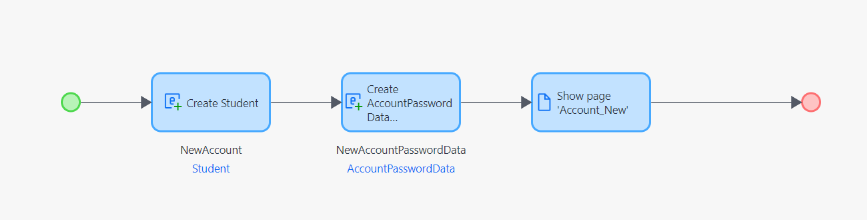
\includegraphics[width=0.9\textwidth]{UniTask_Mendix/ACT_Account_New}
                    \end{center}
                \end{figure}

                    To microflow καλείται από τη σελίδα \texttt{Account\_Overview} με σκοπό τη δημιουργία ενός νέου χρήστη.\footnote{Το πρόθεμα \texttt{ACT} χρησιμοποιείται στην ονομασία των microflows για να δηλώσει μια ενέργεια (action).}

                    Αρχικά δημιουργούνται δύο στιγμιότυπα τύπου \texttt{Student} και \texttt{AccountPasswordData} με ονόματα \texttt{NewAccount} και \texttt{NewAccountPasswordData} αντίστοιχα. Να σημειωθεί πως το \texttt{NewAccountPasswordData} συσχετίζεται με το \texttt{Student}. Τα αντικείμενα δε γίνονται commit ακόμα στη βάση, καθώς είναι κενά. Στη συνέχεια εμφανίζεται η σελίδα \texttt{Account\_New} με τα αντικείμενα \texttt{NewAccount} και \texttt{NewAccountPasswordData} ως Parameters.

                \begin{figure}[H] \noindent
                    \paragraph{\texttt{ACT\_Account\_Save}}
                    \begin{center}
                        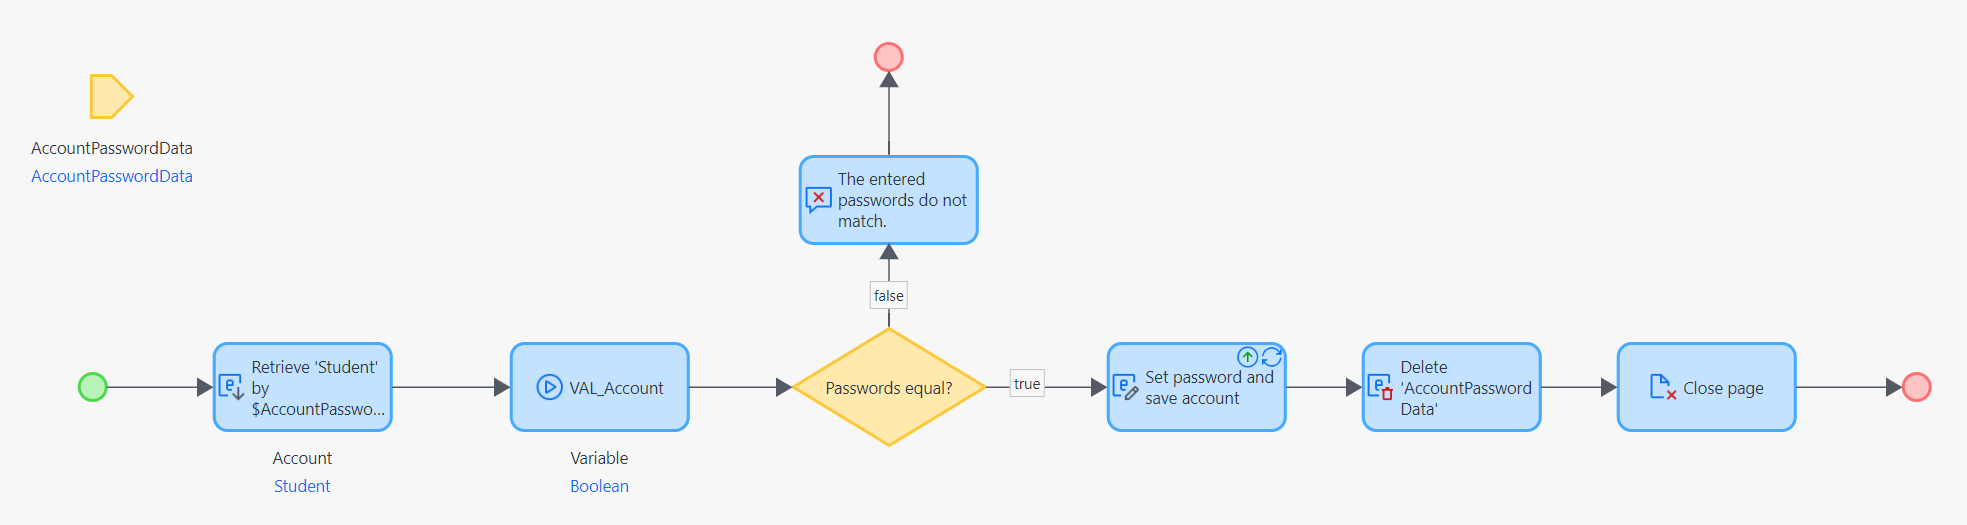
\includegraphics[width=0.9\textwidth]{UniTask_Mendix/ACT_Account_Save}
                    \end{center}
                \end{figure}

                    To microflow καλείται από τη σελίδα \texttt{Account\_New} με σκοπό την αποθήκευση των τιμών του νέου χρήστη.

                    Το microflow έχει ως Parameter το \texttt{AccountPasswordData}. Μαζί με αυτό, ανακτάται το \texttt{Student} αφού συσχετίζονται, και καλείται το microflow \texttt{VAL\_Account} το οποίο ελέγχει αν το \texttt{Name} του \texttt{Student} είναι κενό. Αν το \texttt{Name} είναι κενό, τότε εμφανίζεται ένα popout μήνυμα και το microflow τερματίζεται. Αν το \texttt{Name} δεν είναι κενό, τότε ελέγχεται αν το \texttt{NewPassword} του \texttt{AccountPasswordData} είναι ίσο με το \texttt{ConfirmPassword}, όπως έχουν δοθεί στη φόρμα \texttt{Account\_New}. Αν η συνθήκη δεν ισχύει, τότε εμφανίζεται ένα popout μήνυμα και το microflow τερματίζεται. Αν η συνθήκη ισχύει, τότε το \texttt{NewPassword} γίνεται commit στο \texttt{Account} τύπου \texttt{Student} στο γνώρισμα \texttt{Password} το οποίο είναι Hashed string. Στη συνέχεια το αντικείμενο \texttt{AccountPasswordData} διαγράφεται και κλείνει η σελίδα.

                \begin{figure}[H] \noindent
                    \paragraph{\texttt{ACT\_Account\_Edit}}
                    \begin{center}
                        
\includegraphics[width=0.9\textwidth]{UniTask_Mendix/ACT_Account_Edit}
                    \end{center}
                \end{figure}

                    To microflow καλείται από τη σελίδα \texttt{Account\_Overview} με σκοπό την επεξεργασία ενός υπάρχοντος χρήστη.

                    Το microflow εμφανίζει τη σελίδα \texttt{Account\_Edit} με το \texttt{Account} τύπου \texttt{Student} ως Parameter.

                \begin{figure}[H] \noindent
                    \paragraph{\texttt{VAL\_Password}}
                    \begin{center}
                        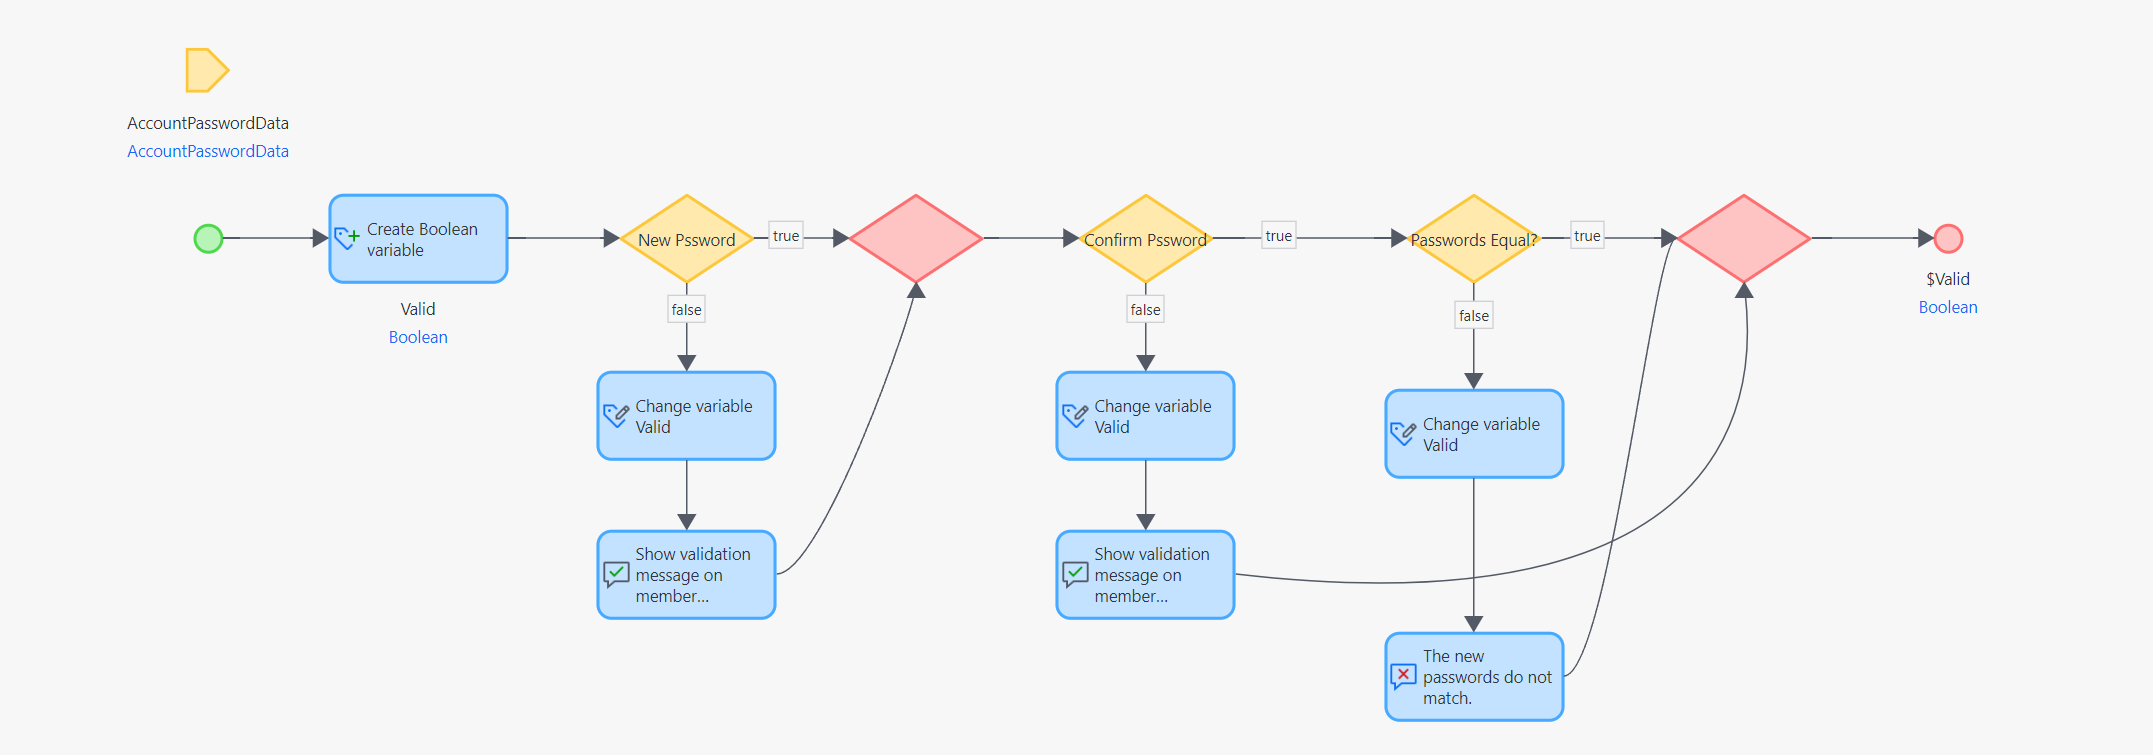
\includegraphics[width=0.9\textwidth]{UniTask_Mendix/VAL_Password}
                    \end{center}
                \end{figure}

                    To microflow καλείται από το microflow \texttt{ChangePassword} με σκοπό τον έλεγχο των συνθηκών για την αλλαγή του κωδικού πρόσβασης.

                    Αρχικά δημιουργείται μια boolean μεταβλητή \texttt{Valid} με αρχική τιμή \texttt{True}. Στη συνέχεια ελέγχεται αν για το \texttt{NewPassword} του αντικειμένου \texttt{AccountPasswordData} ισχύει η συνθήκη (\verb|trim($AccountPasswordData/NewPassword) != ''|). Η έκφραση στη συνθήκη ελέγχει αν έχει δοθεί όντως νέος κωδικός στη φόρμα της σελίδας \texttt{Change\_Password}. Αν η συνθήκη ισχύει, ελέγχεται με παρόμοιο τρόπο και το \texttt{ConfirmPassword} όπως επίσης και το αν είναι ίσο με το \texttt{NewPassword}. Αν κάποια συνθήκη από τις προαναφερθείσες δεν ισχύει, η μεταβλητή \texttt{Valid} γίνεται \texttt{False} και εμφανίζεται κατάλληλο popout μήνυμα. Αν όλες οι συνθήκες ισχύουν, τότε η μεταβλητή \texttt{Valid} παραμένει \texttt{True} και επιστρέφεται από το microflow.

                \begin{figure}[H] \noindent
                    \paragraph{\texttt{ChangePassword}}
                    \begin{center}
                        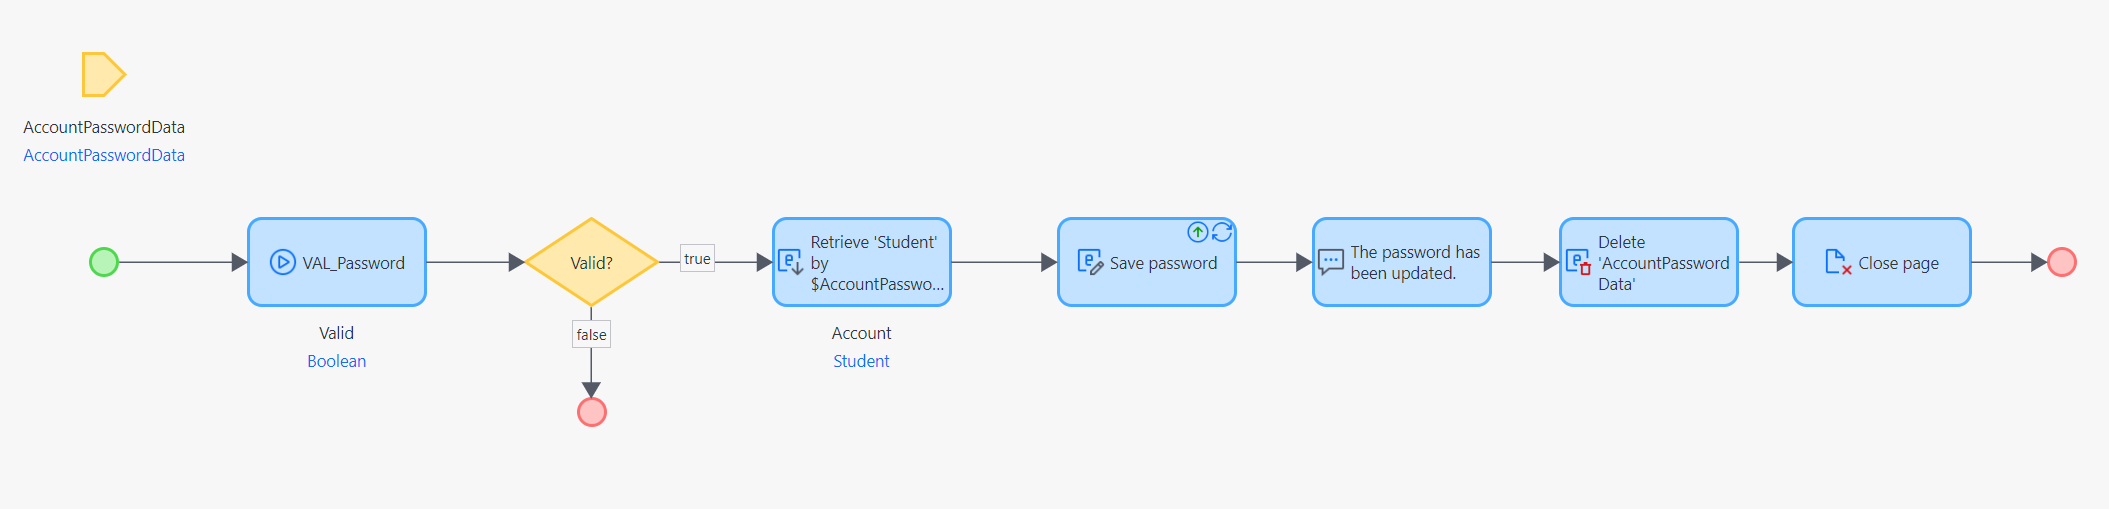
\includegraphics[width=0.9\textwidth]{UniTask_Mendix/ChangePassword}
                    \end{center}
                \end{figure}

                    To microflow καλείται από τη σελίδα \texttt{Change\_Password} με σκοπό την αποθήκευση του νέου κωδικού πρόσβασης για έναν υπάρχων χρήστη.

                    Το microflow έχει ως Parameter το \texttt{AccountPasswordData}. Στην αρχή καλείται το microflow \texttt{VAL\_Password} για τον έλεγχο των συνθηκών. Αν η μεταβλητή \texttt{Valid} που επιστρέφεται από το microflow είναι \texttt{False}, τότε το microflow τερματίζεται. Αν είναι \texttt{True}, τότε γίνεται retrieve και το αντικείμενο \texttt{Student} ως συσχέτιση, γίνεται commit το \texttt{NewPassword} ως Hashed string \texttt{Password} στο \texttt{Student}, εμφανίζεται κατάλληλο popout μήνυμα, διαγράφεται το \texttt{AccountPasswordData} και κλείνει η σελίδα.

                \begin{figure}[H] \noindent
                    \paragraph{\texttt{ACT\_Password\_Change}}
                    \begin{center}
                        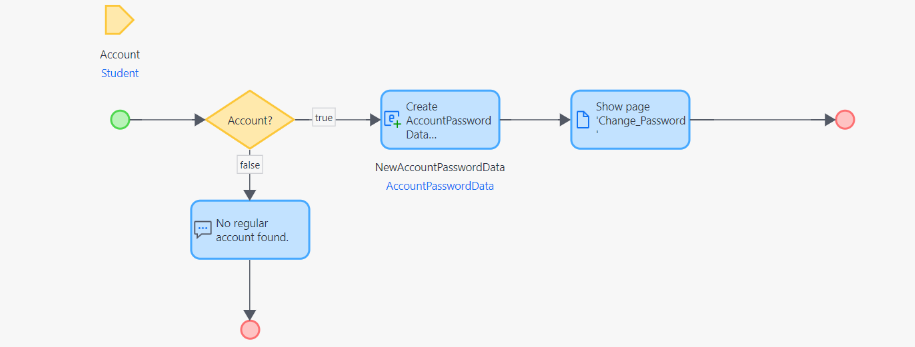
\includegraphics[width=0.9\textwidth]{UniTask_Mendix/ACT_Password_Change}
                    \end{center}
                \end{figure}

                    To microflow καλείται από τη σελίδα \texttt{Account\_Edit} με σκοπό την αλλαγή του κωδικού πρόσβασης ενός υπάρχοντος χρήστη.

                    Με Parameter το \texttt{Account} τύπου \texttt{Student}, αρχικά ελέγχεται αν υπάρχει όντως κάποιο υπαρκτό \texttt{Account}. Αν δεν υπάρχει, εμφανίζεται popout μήνυμα και το microflow τερματίζεται. Αν υπάρχει, τότε δημιουργείται ένα νέο αντικείμενο \texttt{AccountPasswordData} συσχετισμένο με το \texttt{Account} και εμφανίζεται η σελίδα \texttt{Change\_Password} με το \linebreak \texttt{AccountPasswordData} και \texttt{Account} ως Parameters.

                \begin{figure}[H] \noindent
                    \paragraph{\texttt{ASU\_Administrator\_Create}}
                    \begin{center}
                        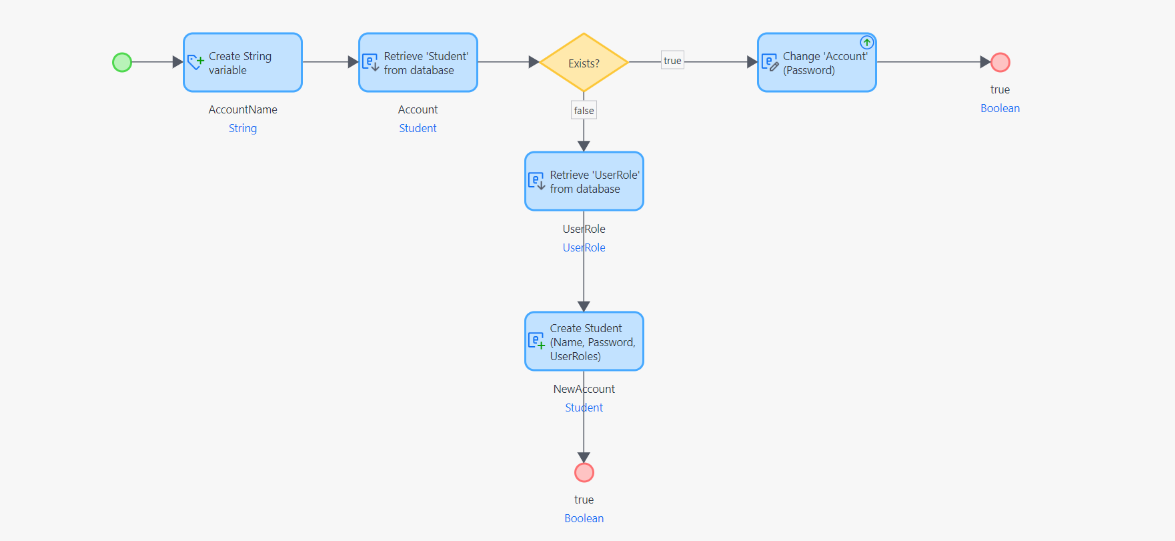
\includegraphics[width=0.9\textwidth]{UniTask_Mendix/ASU_Administrator_Create}
                    \end{center}
                \end{figure}

                    Microflow που καλείται κατά την αρχικοποίηση της εφαρμογής για τη δημιουργία του διαχειριστή της εφαρμογής. \footnote{Το πρόθεμα \texttt{ASU} (After Startup) χρησιμοποιείται στην ονομασία των microflows για να δηλώσει ότι καλείται αμέσως μετά την εκκίνηση της εφαρμογής.}

                    Αρχικά δημιουργείται το String \texttt{AccountName} με τιμή \texttt{'admin'} με το username του διαχειριστή. Στη συνέχεια γίνεται retrieve από τη βάση δεδομένων το \texttt{Student} που έχει ως \texttt{Name} το \texttt{AccountName}. Αν δεν υπάρχει τέτοιος λογαριασμός, τότε γίνονται retrieve τα \texttt{System.UserRoles} και δημιουργείται ένα νέο αντικείμενο \texttt{Student} με \texttt{Name} το \texttt{AccountName}, \texttt{Password} η τιμή \texttt{'admin'} και \texttt{UserRole} το \texttt{UserRole}. Αν υπάρχει ήδη λογαριασμός με το \texttt{AccountName}, τότε αλλάζει ο κωδικός σε \texttt{'admin'}. Είναι προφανές ότι τα στοιχεία σύνδεσης του διαχειριστή έχουν οριστεί ως \texttt{'admin'} και \texttt{'admin'}.

        \subsection{Module \texttt{TaskManager}}
            Το \texttt{TaskManager} περιλαμβάνει τη λειτουργικότητα που αφορά τη διαχείριση των εργασιών της εφαρμογής. Όλες οι οντότητες του domain model, οι σελίδες και τα microflows του module έχουν δικαιώματα ανάγνωσης και εγγραφής από τον \texttt{User} ρόλο, όπως ορίζεται στο \texttt{Security} της εφαρμογής, με εξαίρεση το \texttt{Custom\_LogIn\_Page} που έχει δικαίωμα ο \texttt{Guest}.

            \subsubsection{Domain model του \texttt{TaskManager}}
                \begin{center}
                    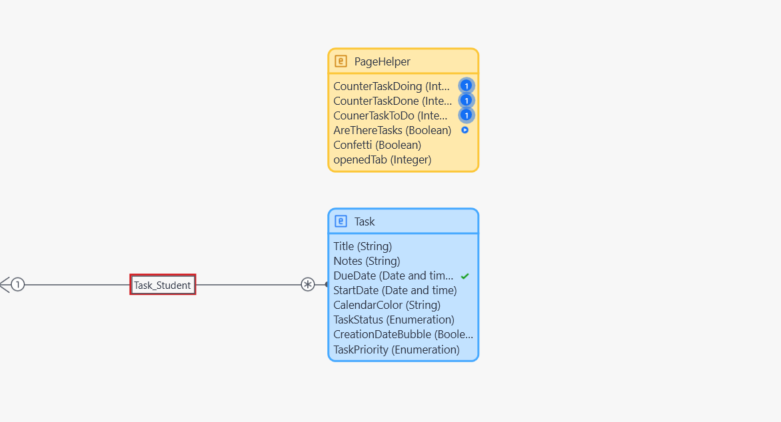
\includegraphics[width=0.9\textwidth]{UniTask_Mendix/TaskManager_DomainModel}
                \end{center}

                Το domain model του \texttt{TaskManager} περιλαμβάνει την οντότητα \texttt{Task} και τη μη-διατηρήσιμη οντότητα \texttt{PageHelper}.

                Η οντότητα \texttt{Task} αναπαριστά την εκάστοτε εργασία του χρήστη της εφαρμογής. Περιλαμβάνει τις ιδιότητες \texttt{Title} τύπου String ως 200 χαρακτήρες με το όνομα της εργασίας, \texttt{Notes} τύπου String με απεριόριστους χαρακτήρες όπου μπορούν να προστεθούν σημειώσεις για αυτή και \texttt{DueDate} τύπου Date and time με την ημερομηνία λήξης. Επίσης, περιλαμβάνει τη \texttt{StartDate} τύπου Date and time με την ημερομηνία έναρξης, η οποία αρχικοποιείται με την τιμή \verb|'%CurrentDateTime%]'| (Token που επιστρέφει την τρέχουσα ημερομηνία και ώρα) και τη \texttt{CalendarColor} τύπου String που αποθηκεύει το χρώμα της εργασίας στο ημερολόγιο. Λόγω της φύσης του widget του ημερολογίου, το String θα έχει πάντα τη μορφή \texttt{'rgb(<0-255>, <0-255>, <0-255>)'} και στην οντότητα αρχικοποιείται με την τιμή \texttt{'rgb(38,74,229)'} που αντιστοιχεί στο μπλε χρώμα.

                Επιπλέον, η οντότητα περιλαμβάνει τις ιδιότητες \texttt{TaskStatus} και \texttt{TaskPriority} όπου είναι Enumeration ιδιότητες των Enumeration εγγράφων \texttt{TaskStatus} και \linebreak \texttt{TaskPriority}, αρχικοποιημένες με \texttt{To\_Do} και \texttt{Low} αντίστοιχα και με την ιδιότητα \texttt{CreationDateBubble} τύπου Boolean που αρχικοποιείται με \texttt{True}. Η ιδιότητα αυτή χρησιμοποιείται για την εμφάνιση ενός επεξηγηματικού μηνύματος στον χρήστη όταν δημιουργεί μια νέα εργασία. Να σημειωθεί επίσης πως το \texttt{DateDue} περιλαμβάνει ένα Validation rule που ελέγχει αν η ημερομηνία λήξης είναι μετά την ημερομηνία έναρξης \texttt{StartDate}, και αν δεν ισχύει, τότε εμφανίζεται κατάλληλο μήνυμα.

                Η οντότητα \texttt{PageHelper} περιλαμβάνει τις ιδιότητες \texttt{CounterTaskDoing}, \linebreak \texttt{CounterTaskDone} και \texttt{CounterTaskToDo} τύπου Integer, των οποίων οι τιμές καθορίζονται από τα microflows \texttt{CounterTaskDoing}, \texttt{CounterTaskDone} και \texttt{CounterTaskToDo} αντίστοιχα. Οι ιδιότητες αυτές χρησιμοποιούνται για την εμφάνιση των τριών μετρητών. Επίσης, περιλαμβάνει την Boolean ιδιότητα \texttt{AreThereTasks} που καθορίζεται από το microflow \texttt{AreThereTasks} και χρησιμεύει για την εμφάνιση του επεξηγηματικού παραθύρου στο Dashboard, την Boolean ιδιότητα \texttt{Confetti} που αρχικοποιείται με \texttt{False} και χρησιμοποιείται για την εμφάνιση του κομφετί (σύστημα επιβράβευσης), και τέλος την ιδιότητα \texttt{openedTab} τύπου Integer αρχικοποιημένη με μηδέν που χρησιμεύει για την αποθήκευση της τρέχουσας καρτέλας του Dashboard που έχει ανοίξει ο χρήστης.

            \subsubsection{Σελίδες του \texttt{TaskManager}}
                Στο \texttt{TaskManager} περιλαμβάνονται οι εξής σελίδες:

                \begin{figure}[H] \noindent
                    \paragraph{\texttt{Account\_Overview}}
                    \begin{center}
                        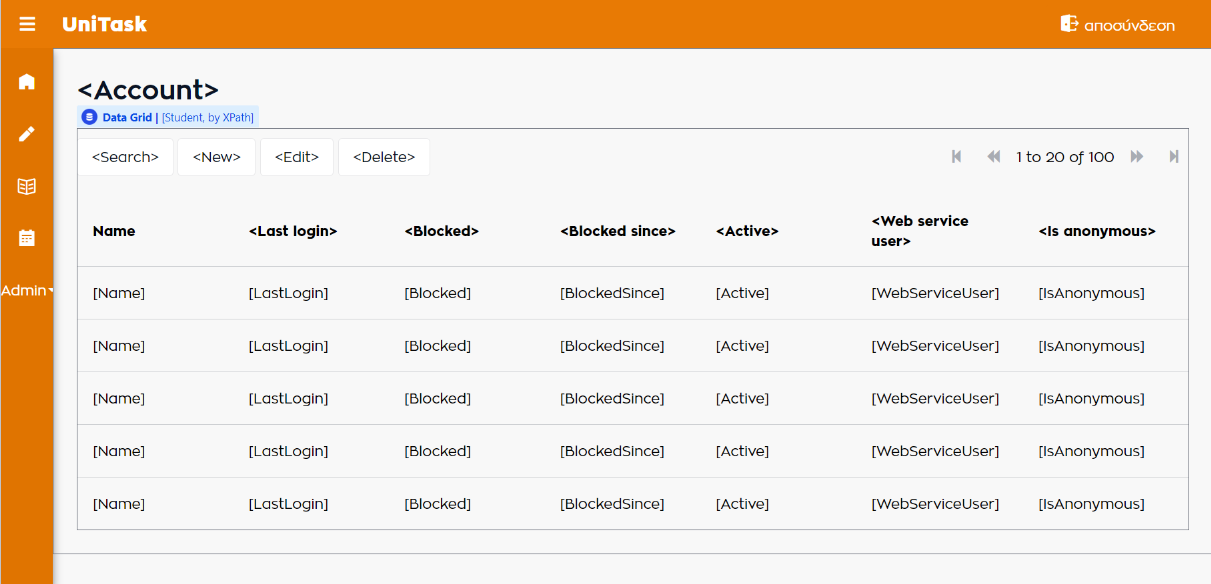
\includegraphics[width=0.9\textwidth]{UniTask_Mendix/Account_Overview}
                    \end{center}
                \end{figure}


            \subsubsection{Microflows του \texttt{TaskManager}}

            \subsubsection{Έγγραφα του \texttt{TaskManager}}